\documentclass[oneside]{VUMIFPSkursinis}
\usepackage{algorithmicx}
\usepackage{algorithm}
\usepackage{algpseudocode}
\usepackage{amsfonts}
\usepackage{float}
\usepackage{amsmath}
\usepackage{bm}
\usepackage{caption}
\usepackage{color}
\usepackage{float}
\usepackage{graphicx}
\usepackage{listings}
\usepackage{subfig}
\usepackage{ltablex}
\usepackage{longtable}
\usepackage{wrapfig}
\usepackage{subfig}
\usepackage{pbox}
\renewcommand{\labelenumii}{\theenumii}
\renewcommand{\theenumii}{\theenumi.\arabic{enumii}.}
\renewcommand{\labelenumiii}{\theenumiii}
\renewcommand{\theenumiii}{\theenumii\arabic{enumiii}.}
\newcolumntype{P}[1]{>{\centering\arraybackslash}p{#1}}
\usepackage[%  
    colorlinks=true,
    linkcolor=black
]{hyperref}
\university{Vilniaus universitetas}
\faculty{Matematikos ir informatikos fakultetas}
\department{Programų sistemų katedra}
\papertype{Programų sistemų inžinerija II laboratorinis darbas II}
\title{Reikalavimų analizė ir techninė architektūra}
\titleineng{Requirements Analysis and Technical Architecture}
\status{2 kurso 3 grupės studentai}



\supervisor{Audronė Lupeikienė, M. Darbuot., Dr.}
\date{Vilnius – \the\year}

\bibliography{bibliografija}

\begin{document}
\maketitle
\tableofcontents

\section{Anotacija}
\begin{itemize}
	\item{Matas Savickis}
	\item{Justas Tvarijonas}
	\item{Rytautas Kvasinskas}
	\item{Greta Pyrantaitė}
	\item{Tomas Kiziela}
\end{itemize}

\section{Sistemos detalus projektas}
	\subsection{Sistemos užduotys}
		\subsubsection{Užduočių diagramos}


			\begin{figure}[h]
    				\centering
    				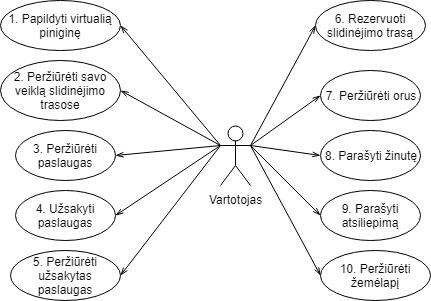
\includegraphics[width=0.75\textwidth]{useCaseVartotojas.png}
    				\caption{Vartotojo užduočių diagrama}
    				\label{fig:VartotojoUseCasel}
			\end{figure}

			\begin{figure}[h]
    				\centering
    				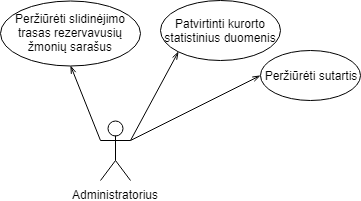
\includegraphics[width=0.75\textwidth]{useCaseAdministratorius.png}
    				\caption{Administratoriaus užduočių diagrama}
    				\label{fig:AdministratoriausUseCasel}
			\end{figure}
\pagebreak

	\subsubsection{Robastiškumo diagramos}

			\begin{figure}[h]
    				\centering
    				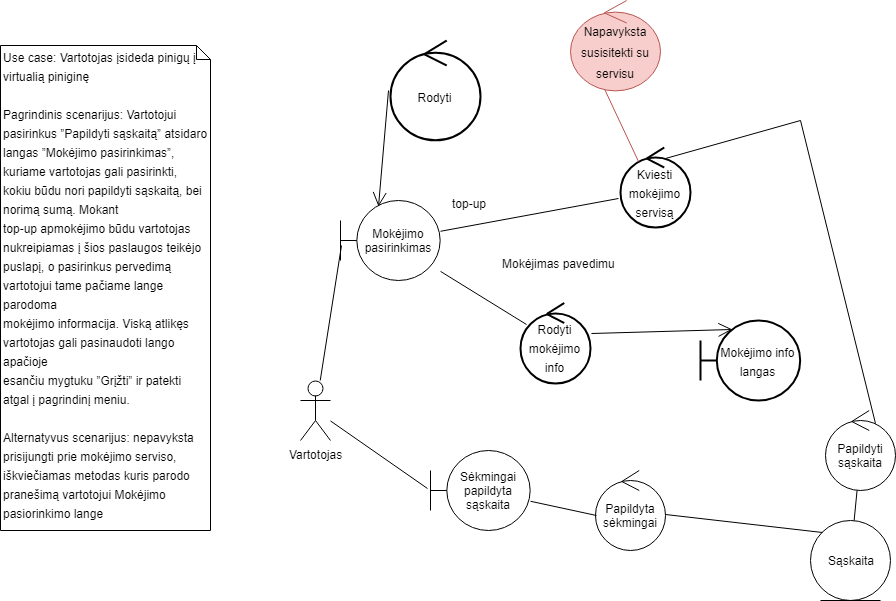
\includegraphics[width=1\textwidth]{rob1.png}
    				\caption{Vartotojas įsideda pinigų į virtualią piniginę}
    				\label{fig:Vartotojas įsideda pinigų į virtualią piniginę}
			\end{figure}

			\begin{figure}[h]
    				\centering
    				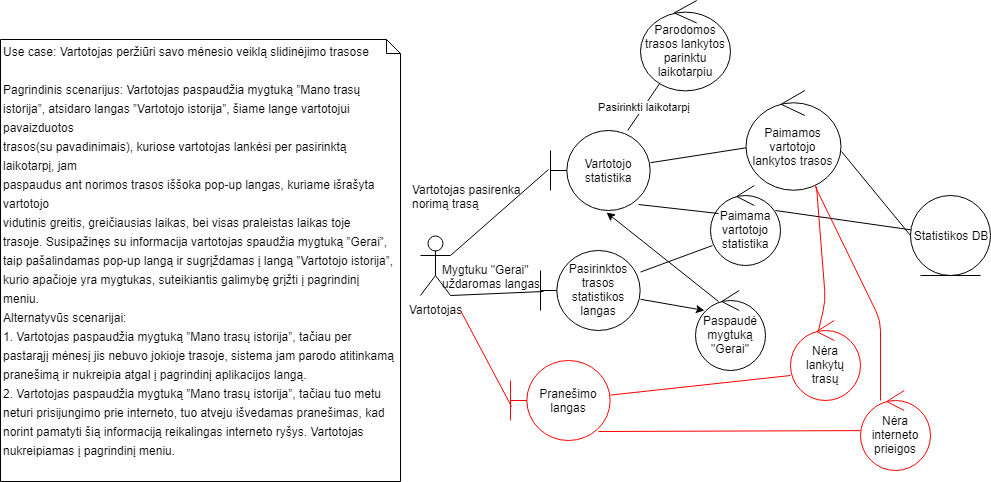
\includegraphics[width=1\textwidth]{rob2.png}
    				\caption{Vartotojas peržiūri savo veiklą trasose}
    				\label{fig:Vartotojas peržiūri savo veiklą trasose}
			\end{figure}

			\begin{figure}[h]
    				\centering
    				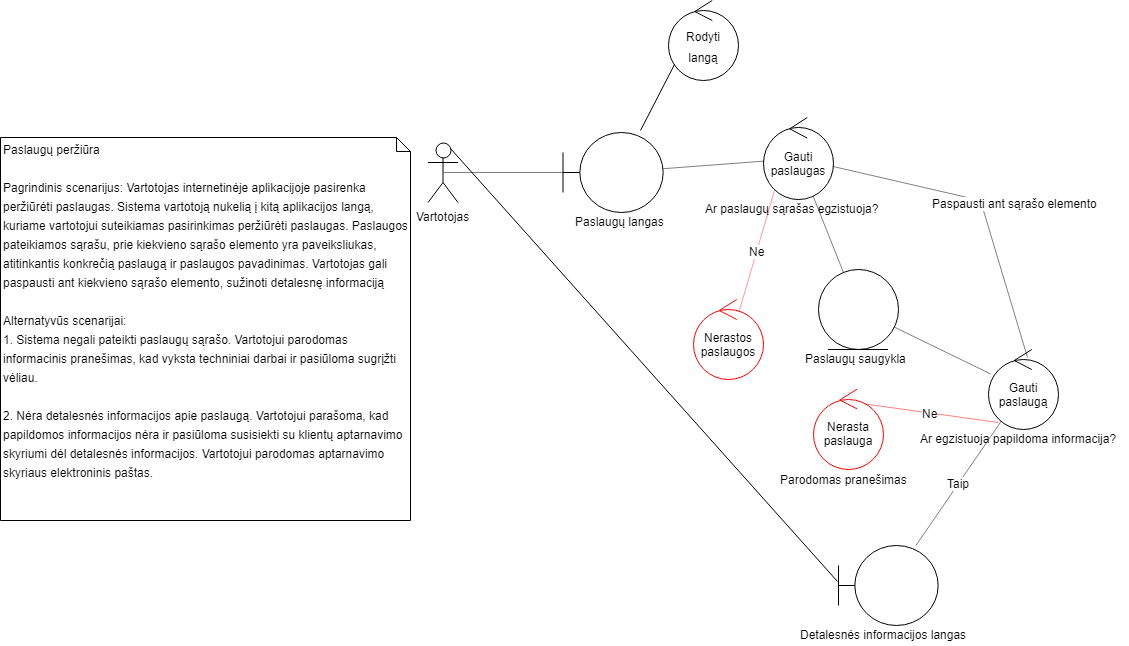
\includegraphics[width=1\textwidth]{rob4.png}
    				\caption{Paslaugų peržiūra}
    				\label{fig:Paslaugų peržiūra}
			\end{figure}

			\begin{figure}[h]
    				\centering
    				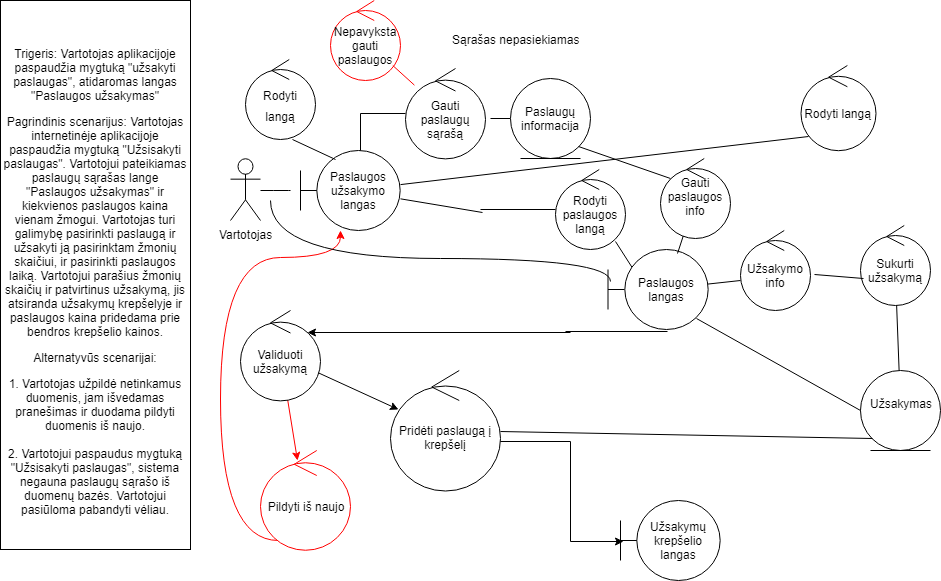
\includegraphics[width=1\textwidth]{rob6.png}
    				\caption{Vartotojas užsisako paslaugas}
    				\label{fig:Vartotojas užsisako paslaugas}
			\end{figure}

			\begin{figure}[h]
    				\centering
    				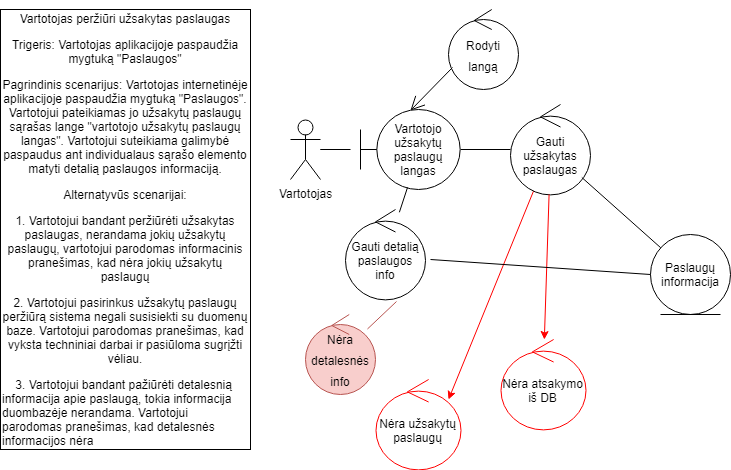
\includegraphics[width=1\textwidth]{rob7.png}
    				\caption{Vartotojas peržiūri užsakytas paslaugas}
    				\label{fig:Vartotojas peržiūri užsakytas paslaugas}
			\end{figure}

			\begin{figure}[h]
    				\centering
    				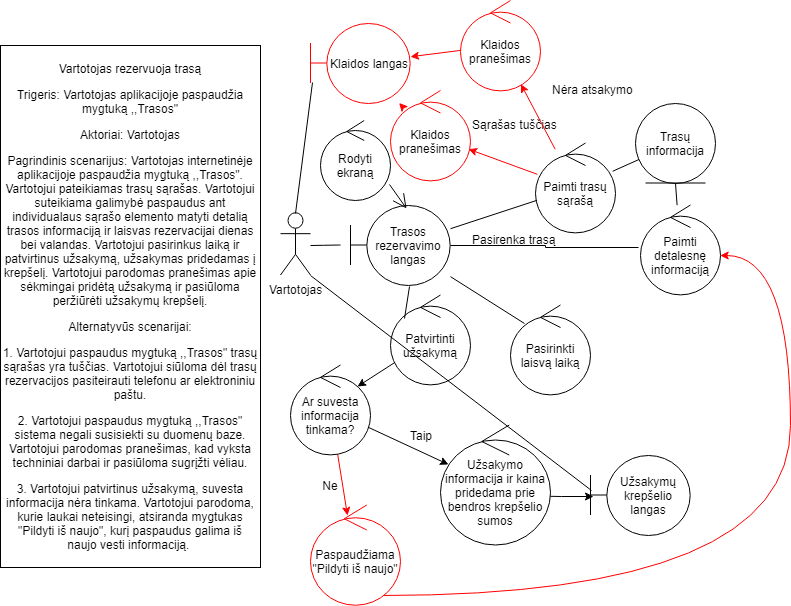
\includegraphics[width=1\textwidth]{rob8.png}
    				\caption{Vartotojas rezervuoja trasą}
    				\label{fig:VartotojoUseCasel}
			\end{figure}

			\begin{figure}[h]
    				\centering
    				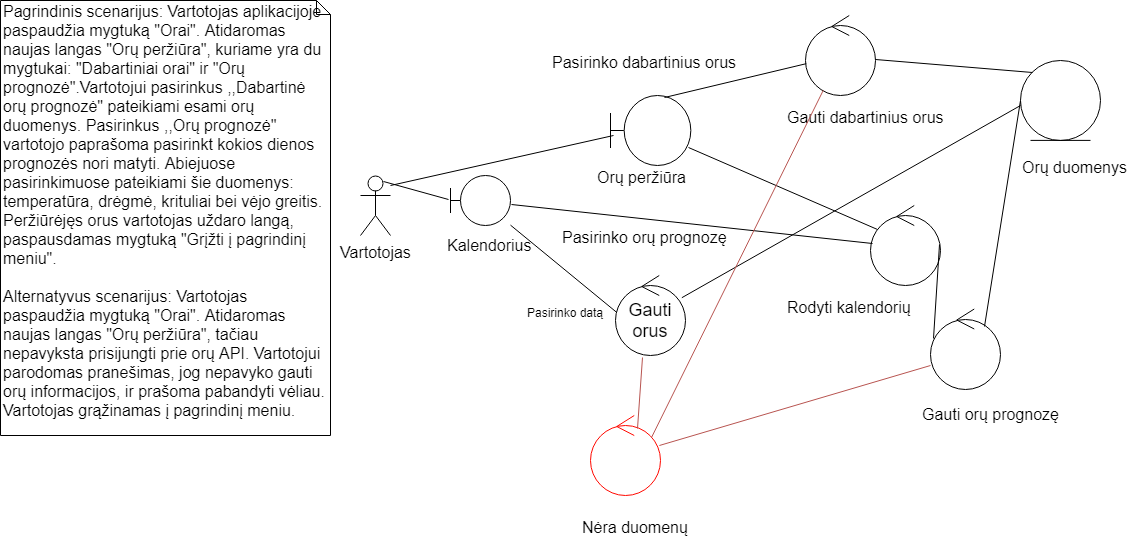
\includegraphics[width=1\textwidth]{rob10.png}
    				\caption{Vartotojas peržiūri orų prognozę}
    				\label{fig:Vartotojas peržiūri orų prognozę}
			\end{figure}

			\begin{figure}[h]
    				\centering
    				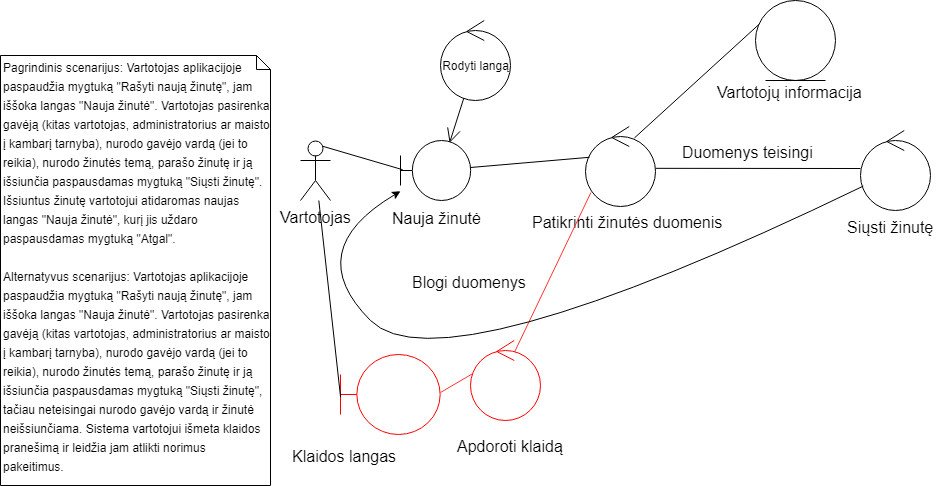
\includegraphics[width=1\textwidth]{rob11.png}
    				\caption{Vartotojas rašo žinutę}
    				\label{fig:Vartotojas rašo žinutę}
			\end{figure}

			\begin{figure}[h]
    				\centering
    				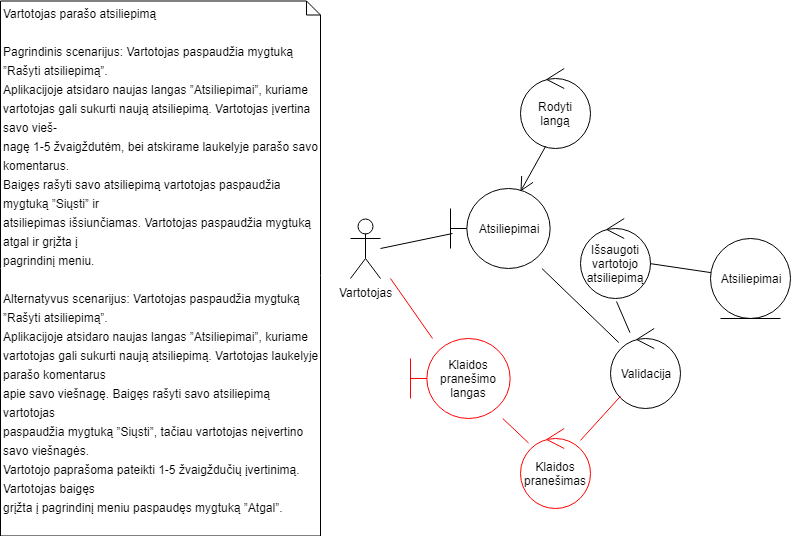
\includegraphics[width=1\textwidth]{rob12.png}
    				\caption{Vartotojas rašo atsiliepimą}
    				\label{fig:Vartotojas rašo atsiliepimą}
			\end{figure}

			\begin{figure}[h]
    				\centering
    				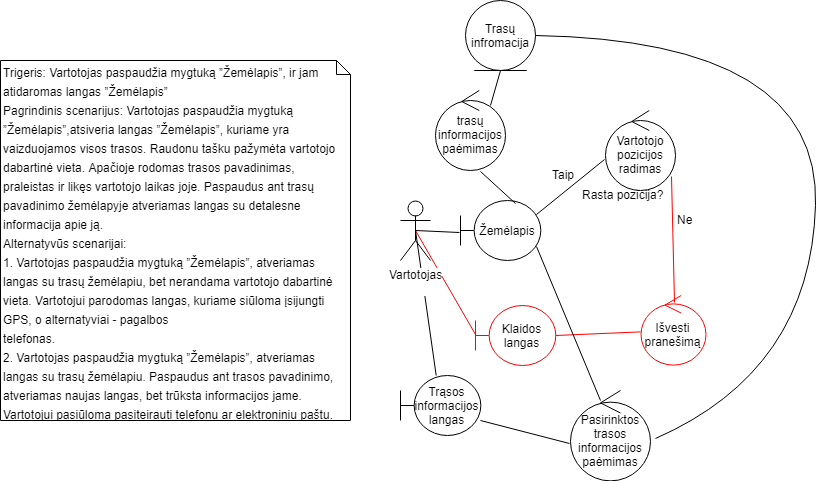
\includegraphics[width=1\textwidth]{rob13.png}
    				\caption{Vartotojas peržiūri žemėlapį}
    				\label{fig:Vartotojas peržiūri žemėlapį}
			\end{figure}

			\begin{figure}[h]
    				\centering
    				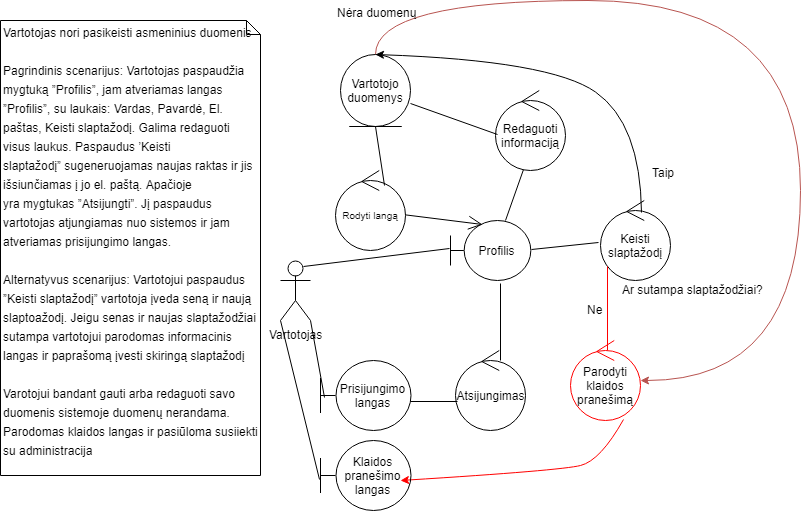
\includegraphics[width=1\textwidth]{rob14.png}
    				\caption{Vartotojas keičia asmeninius duomenis}
    				\label{fig:Vartotojas keičia asmeninius duomenis}
			\end{figure}

\section{Sekų diagramos}
			\begin{figure}[h]
    				\centering
    				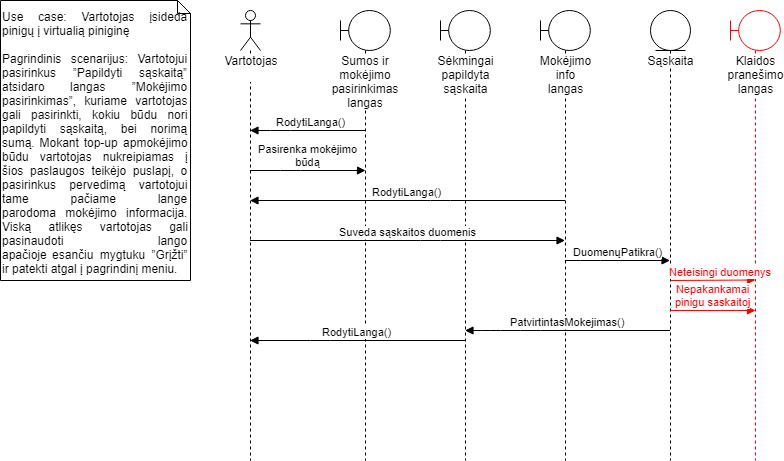
\includegraphics[width=1\textwidth]{seq1.png}
    				\caption{Vartotojas įsideda pinigų į virtualią piniginę}
    				\label{fig:Vartotojas įsideda pinigų į virtualią piniginę}
			\end{figure}

			\begin{figure}[h]
    				\centering
    				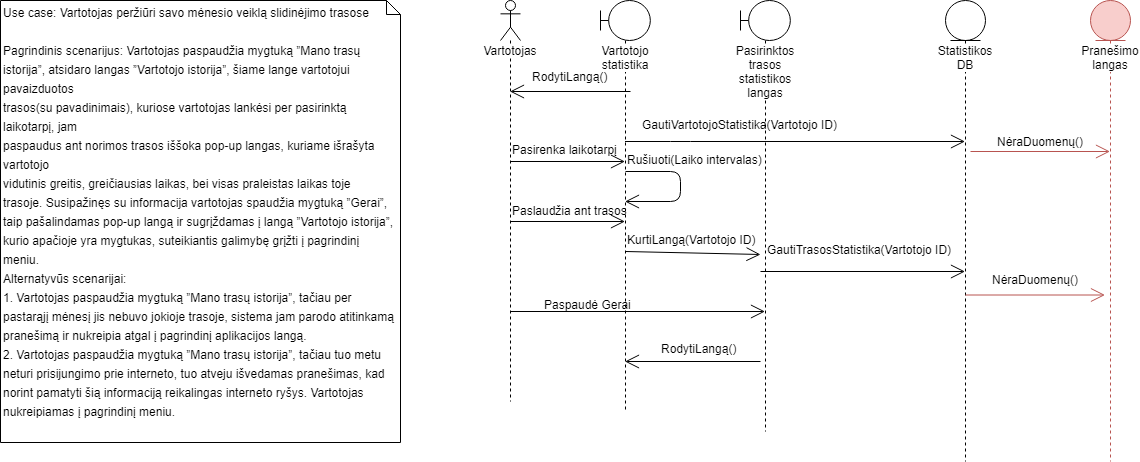
\includegraphics[width=1\textwidth]{seq2.png}
    				\caption{Vartotojas peržiūri savo veiklą trasose}
    				\label{fig:Vartotojas peržiūri savo veiklą trasose}
			\end{figure}


			\begin{figure}[h]
    				\centering
    				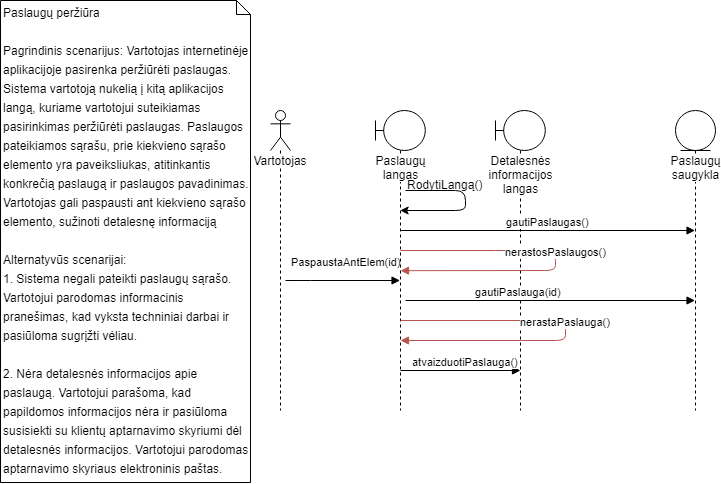
\includegraphics[width=1\textwidth]{seq4.png}
    				\caption{Paslaugų peržiūra}
    				\label{fig:Paslaugų peržiūra}
			\end{figure}

			\begin{figure}[h]
    				\centering
    				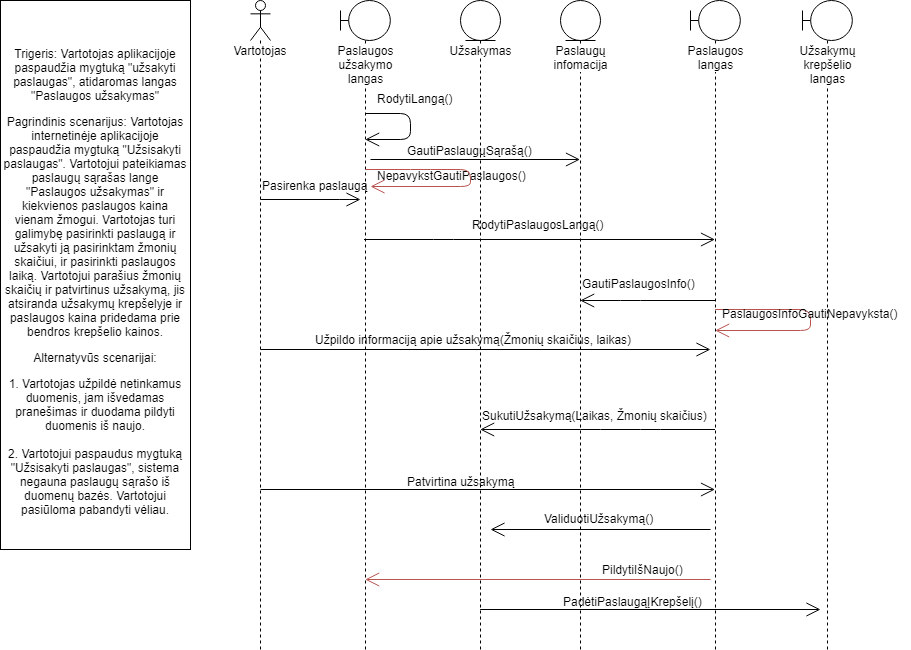
\includegraphics[width=1\textwidth]{seq6.png}
    				\caption{Vartotojas užsisako paslaugas}
    				\label{fig:Vartotojas užsisako paslaugas}
			\end{figure}

			\begin{figure}[h]
    				\centering
    				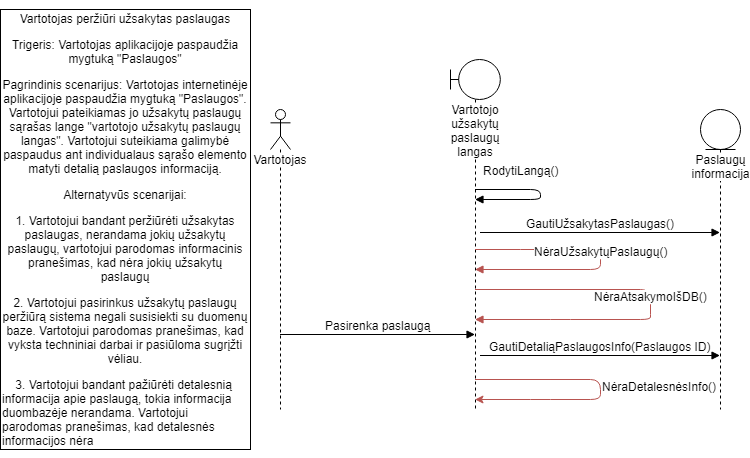
\includegraphics[width=1\textwidth]{seq7.png}
    				\caption{Vartotojas peržiūri užsakytas paslaugas}
    				\label{fig:Vartotojas peržiūri užsakytas paslaugas}
			\end{figure}

			\begin{figure}[h]
    				\centering
    				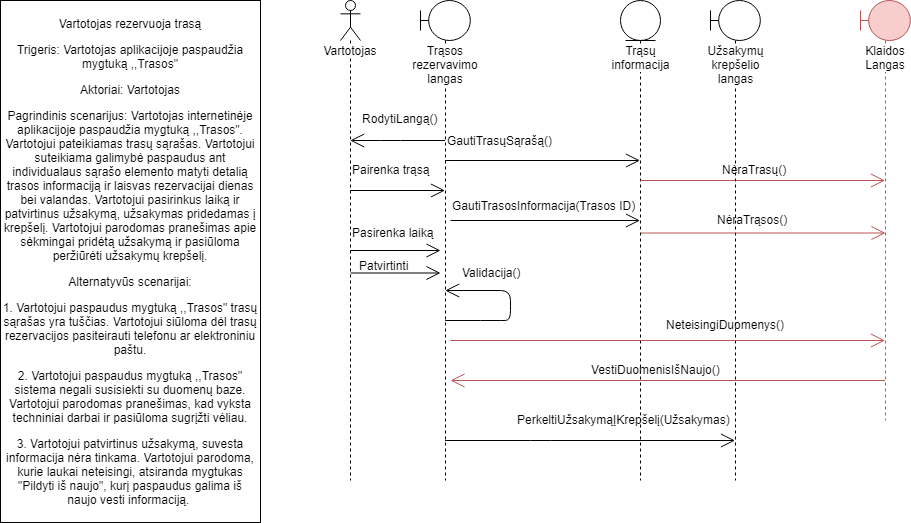
\includegraphics[width=1\textwidth]{seq8.png}
    				\caption{Vartotojas rezervuoja trasą}
    				\label{fig:VartotojoUseCasel}
			\end{figure}

			\begin{figure}[h]
    				\centering
    				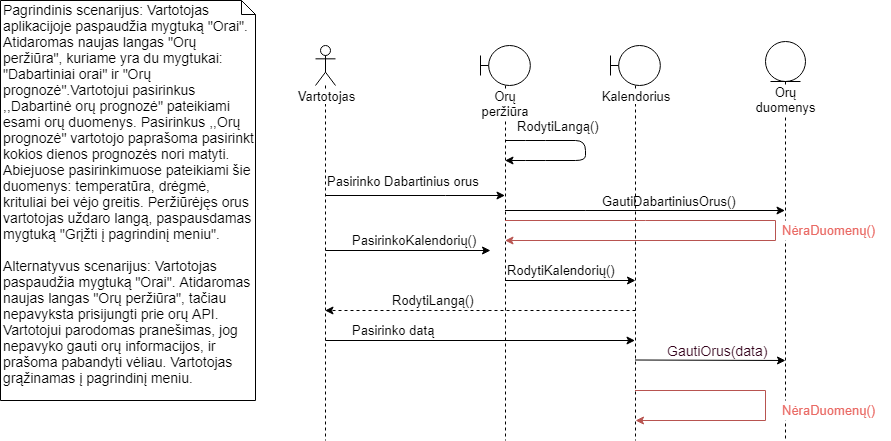
\includegraphics[width=1\textwidth]{seq10.png}
    				\caption{Vartotojas peržiūri orų prognozę}
    				\label{fig:Vartotojas peržiūri orų prognozę}
			\end{figure}

			\begin{figure}[h]
    				\centering
    				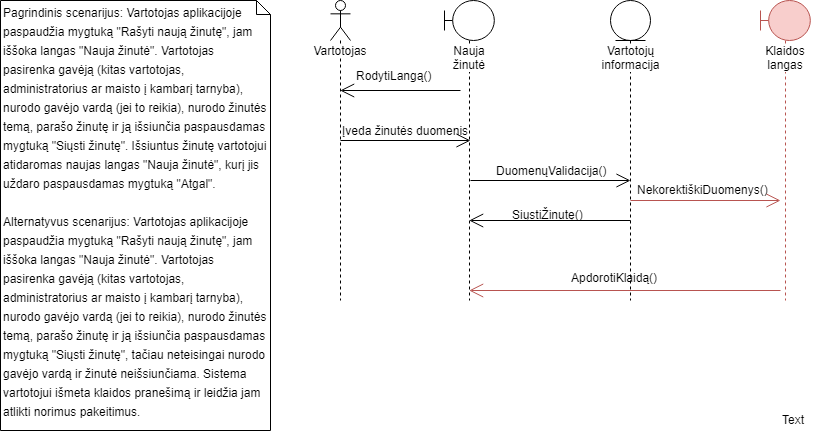
\includegraphics[width=1\textwidth]{seq11.png}
    				\caption{Vartotojas rašo žinutę}
    				\label{fig:Vartotojas rašo žinutę}
			\end{figure}

			\begin{figure}[h]
    				\centering
    				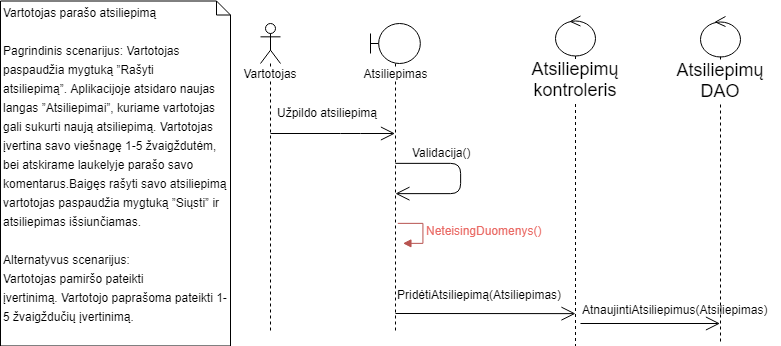
\includegraphics[width=1\textwidth]{seq12.png}
    				\caption{Vartotojas rašo atsiliepimą}
    				\label{fig:Vartotojas rašo atsiliepimą}
			\end{figure}

			\begin{figure}[h]
    				\centering
    				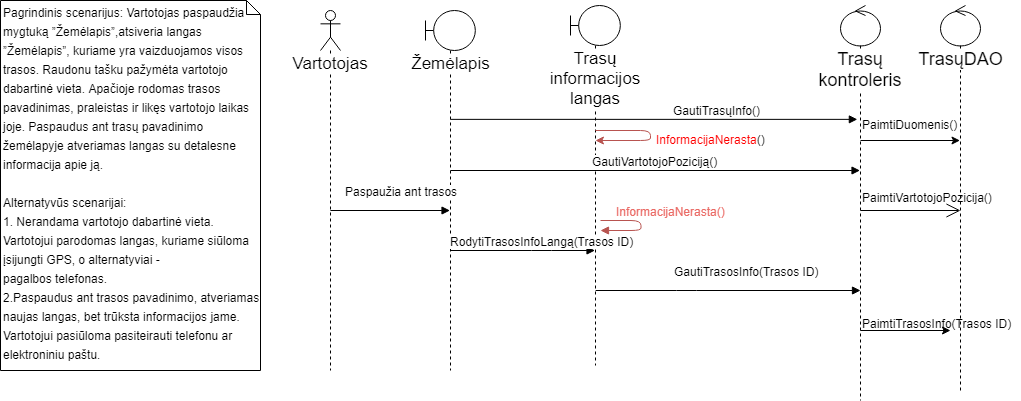
\includegraphics[width=1\textwidth]{seq13.png}
    				\caption{Vartotojas peržiūri žemėlapį}
    				\label{fig:Vartotojas peržiūri žemėlapį}
			\end{figure}

			\begin{figure}[h]
    				\centering
    				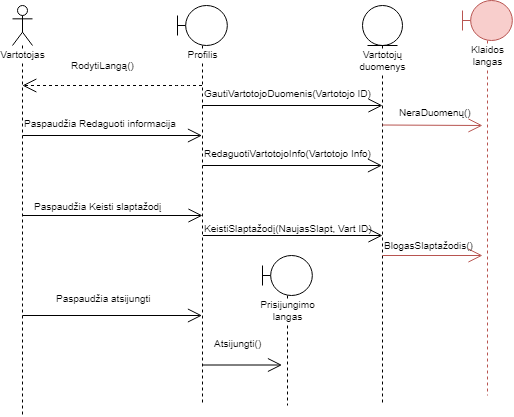
\includegraphics[width=1\textwidth]{seq14.png}
    				\caption{Vartotojas keičia asmeninius duomenis}
    				\label{fig:Vartotojas keičia asmeninius duomenis}
			\end{figure}

\section{Klasių diagrama}

			\begin{figure}[h]
    				\centering
    				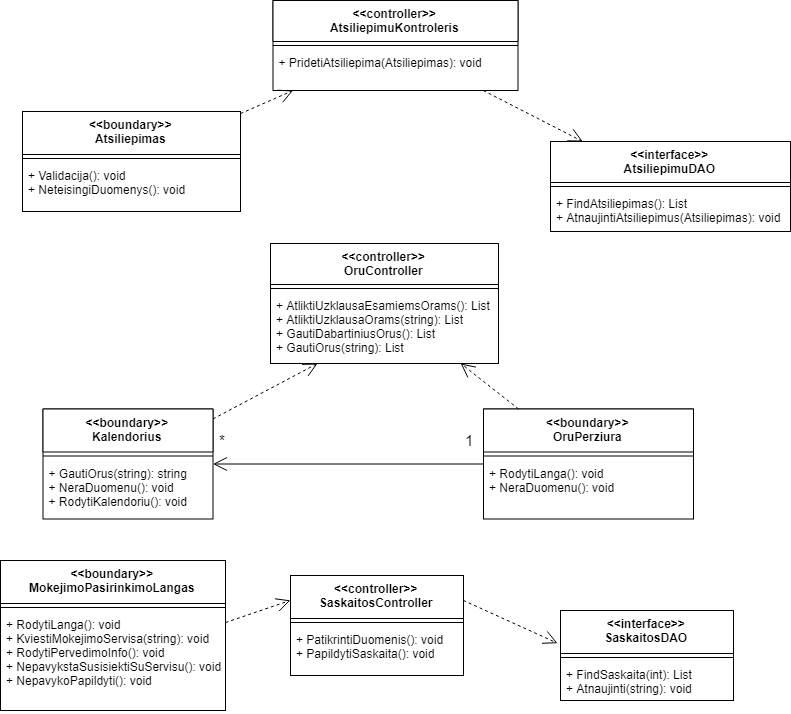
\includegraphics[width=1\textwidth]{classA.png}
    				\caption{Klasių diagrama 1}
    				\label{fig:KlasiuDiagrama}
			\end{figure}
			\begin{figure}[h]
    				\centering
    				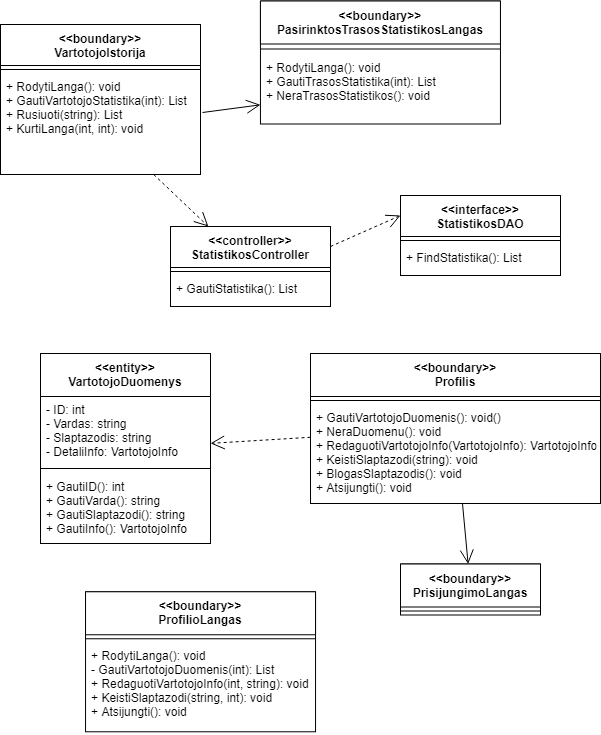
\includegraphics[width=1\textwidth]{classB.png}
    				\caption{Klasių diagrama 2}
    				\label{fig:KlasiuDiagrama}
			\end{figure}
			\begin{figure}[h]
    				\centering
    				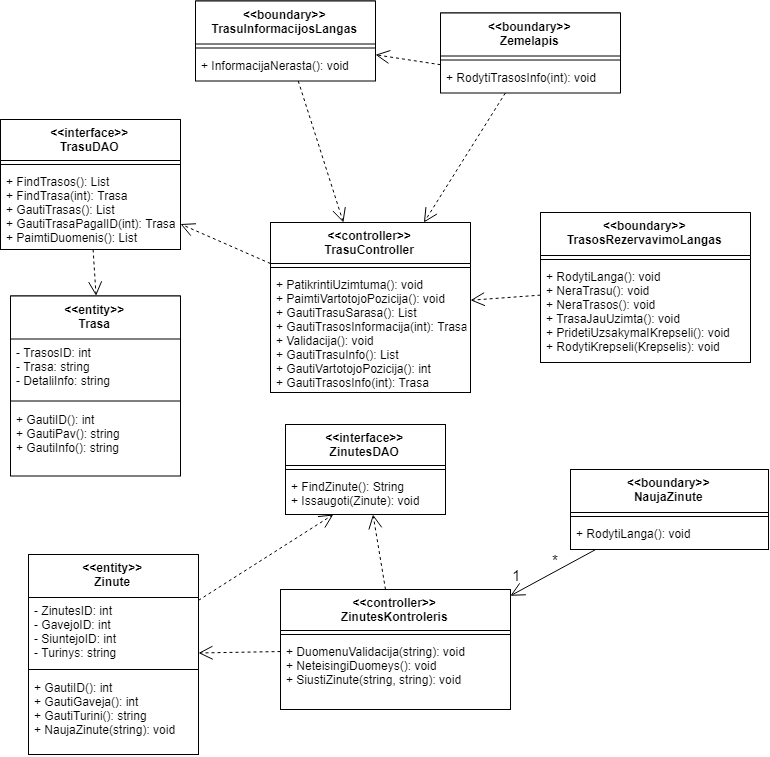
\includegraphics[width=1\textwidth]{classC.png}
    				\caption{Klasių diagrama 3}
    				\label{fig:KlasiuDiagrama}
			\end{figure}
			\begin{figure}[h]
    				\centering
    				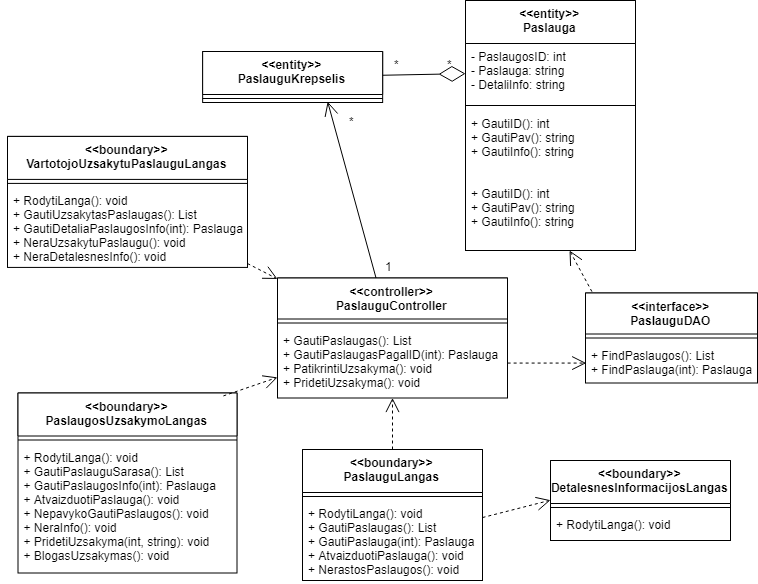
\includegraphics[width=1\textwidth]{classD.png}
    				\caption{Klasių diagrama 4}
    				\label{fig:KlasiuDiagrama}
			\end{figure}

\section{Detalaus projekto peržiūra}
	\subsection{Peržiūra}
Peržiūros metu sutvarkėme savo robastiškumo ir sekų diagramas, kad jos atitiktų viena kitą ir atitiktų use case'us. Pridėjome papildomus alternatyvius scenarijus. Pagrindinis dalykas, kurį pakeitėm yra atskiras langas, kuris atsiranda įvykus nenumatytam scenarijui. Dabar pagal sekų diagramas įvykus alternatyviam scenarijui informacinė žinutė atsiranda tame pačiame lange, kuris buvo atsakingas dėl sukeltos klaidos.  Ištrynėme nereikalingus kontrolerius, kurie nieko nedarė. Panaikinome ,,Ataskaitos" use case'a, nes supratome, kad šis use case'as yra neaiškus ir geriau pagalvojus nebūtinas mūsų sistemai funkcionuoti. Pagal pakeistas sekų diagramas taip pat pakeitėme klasių diagramą. Po peržiūros esame pasiruošę pradėti rašyti kodą. Peržiūrą vykdėme dviem etapais. Pirmame etame kiekvienas komandos narys peržiūrėjo tas diagramas, kurių jis nedarė(svetimas klaidas pastebėti lengviau). Antrame etape susirinko visa komanda ir ėjome po vieną  diagramą aptardami, ar viskas joje gerai, ir padarydami paskutinius pataisymus.
	\subsection{Atsekamumas}
	
	\begin{figure}[h]
    				\centering
    				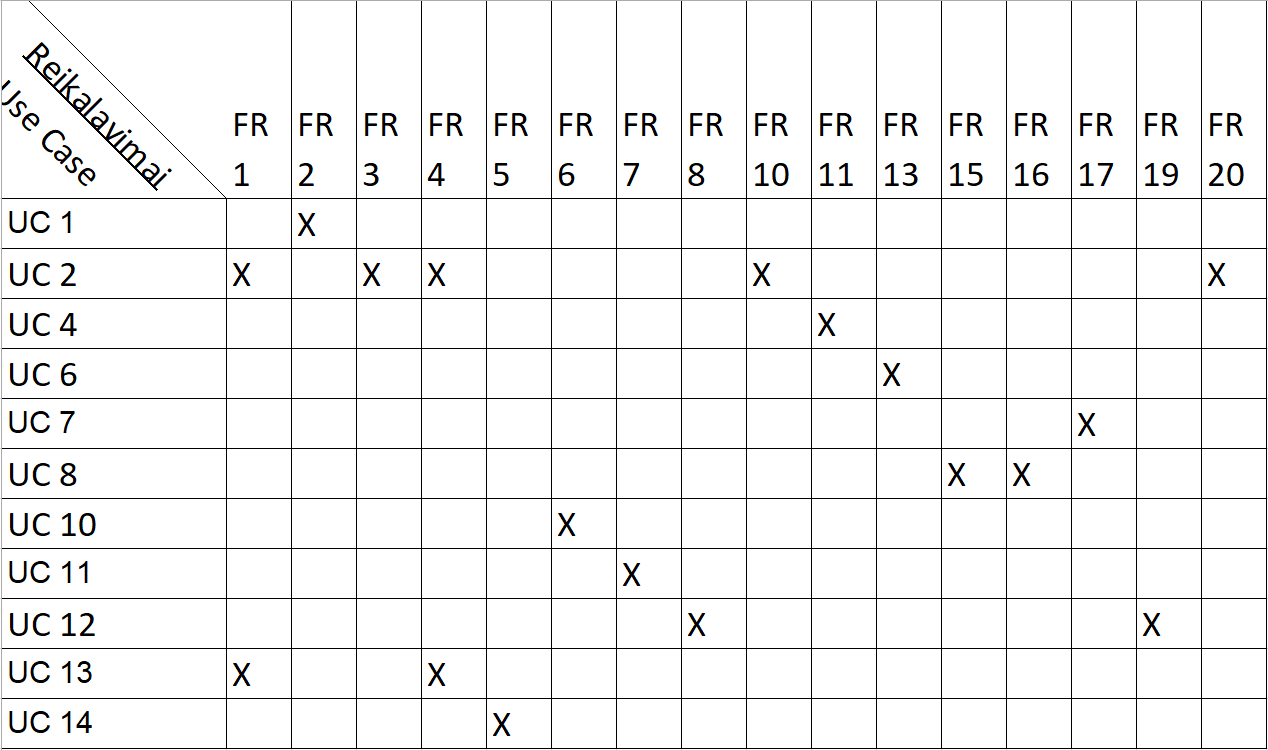
\includegraphics[width=0.75\textwidth]{UCxFR.png}
    				\caption{UC - FR atsekamumas}
			\end{figure}
			
	\begin{figure}[h]
    				\centering
    				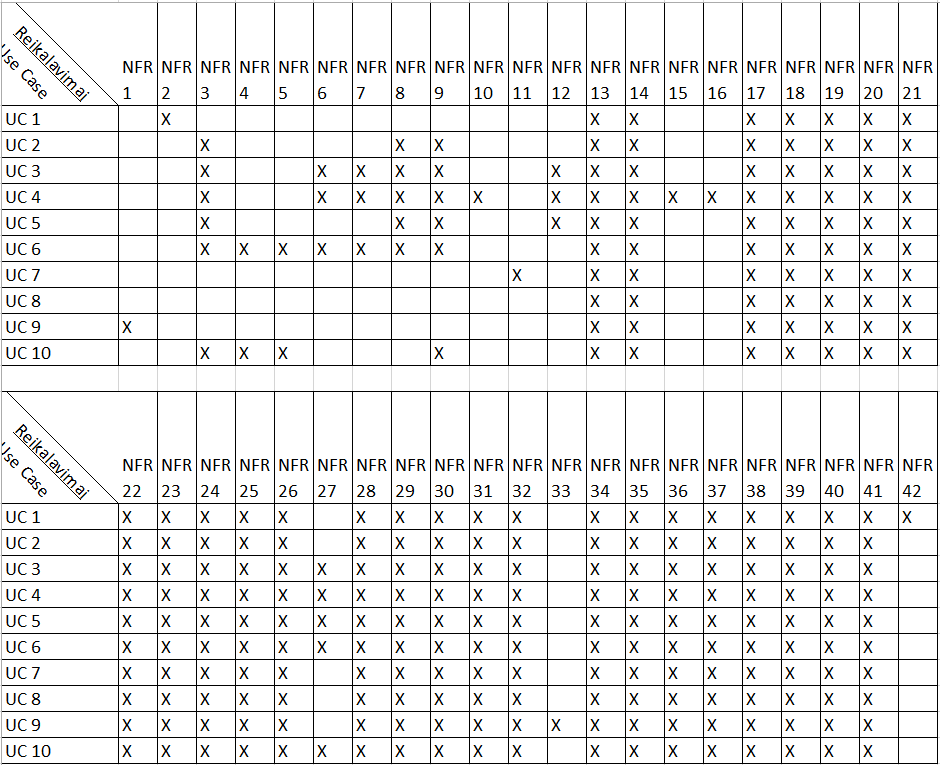
\includegraphics[width=1\textwidth]{UC_NFR.png}
    				\caption{UC - NFR atsekamumas}
			\end{figure}
\section{Testavimo scenarijai}
	
			\begin{figure}[h]
    				\centering
    				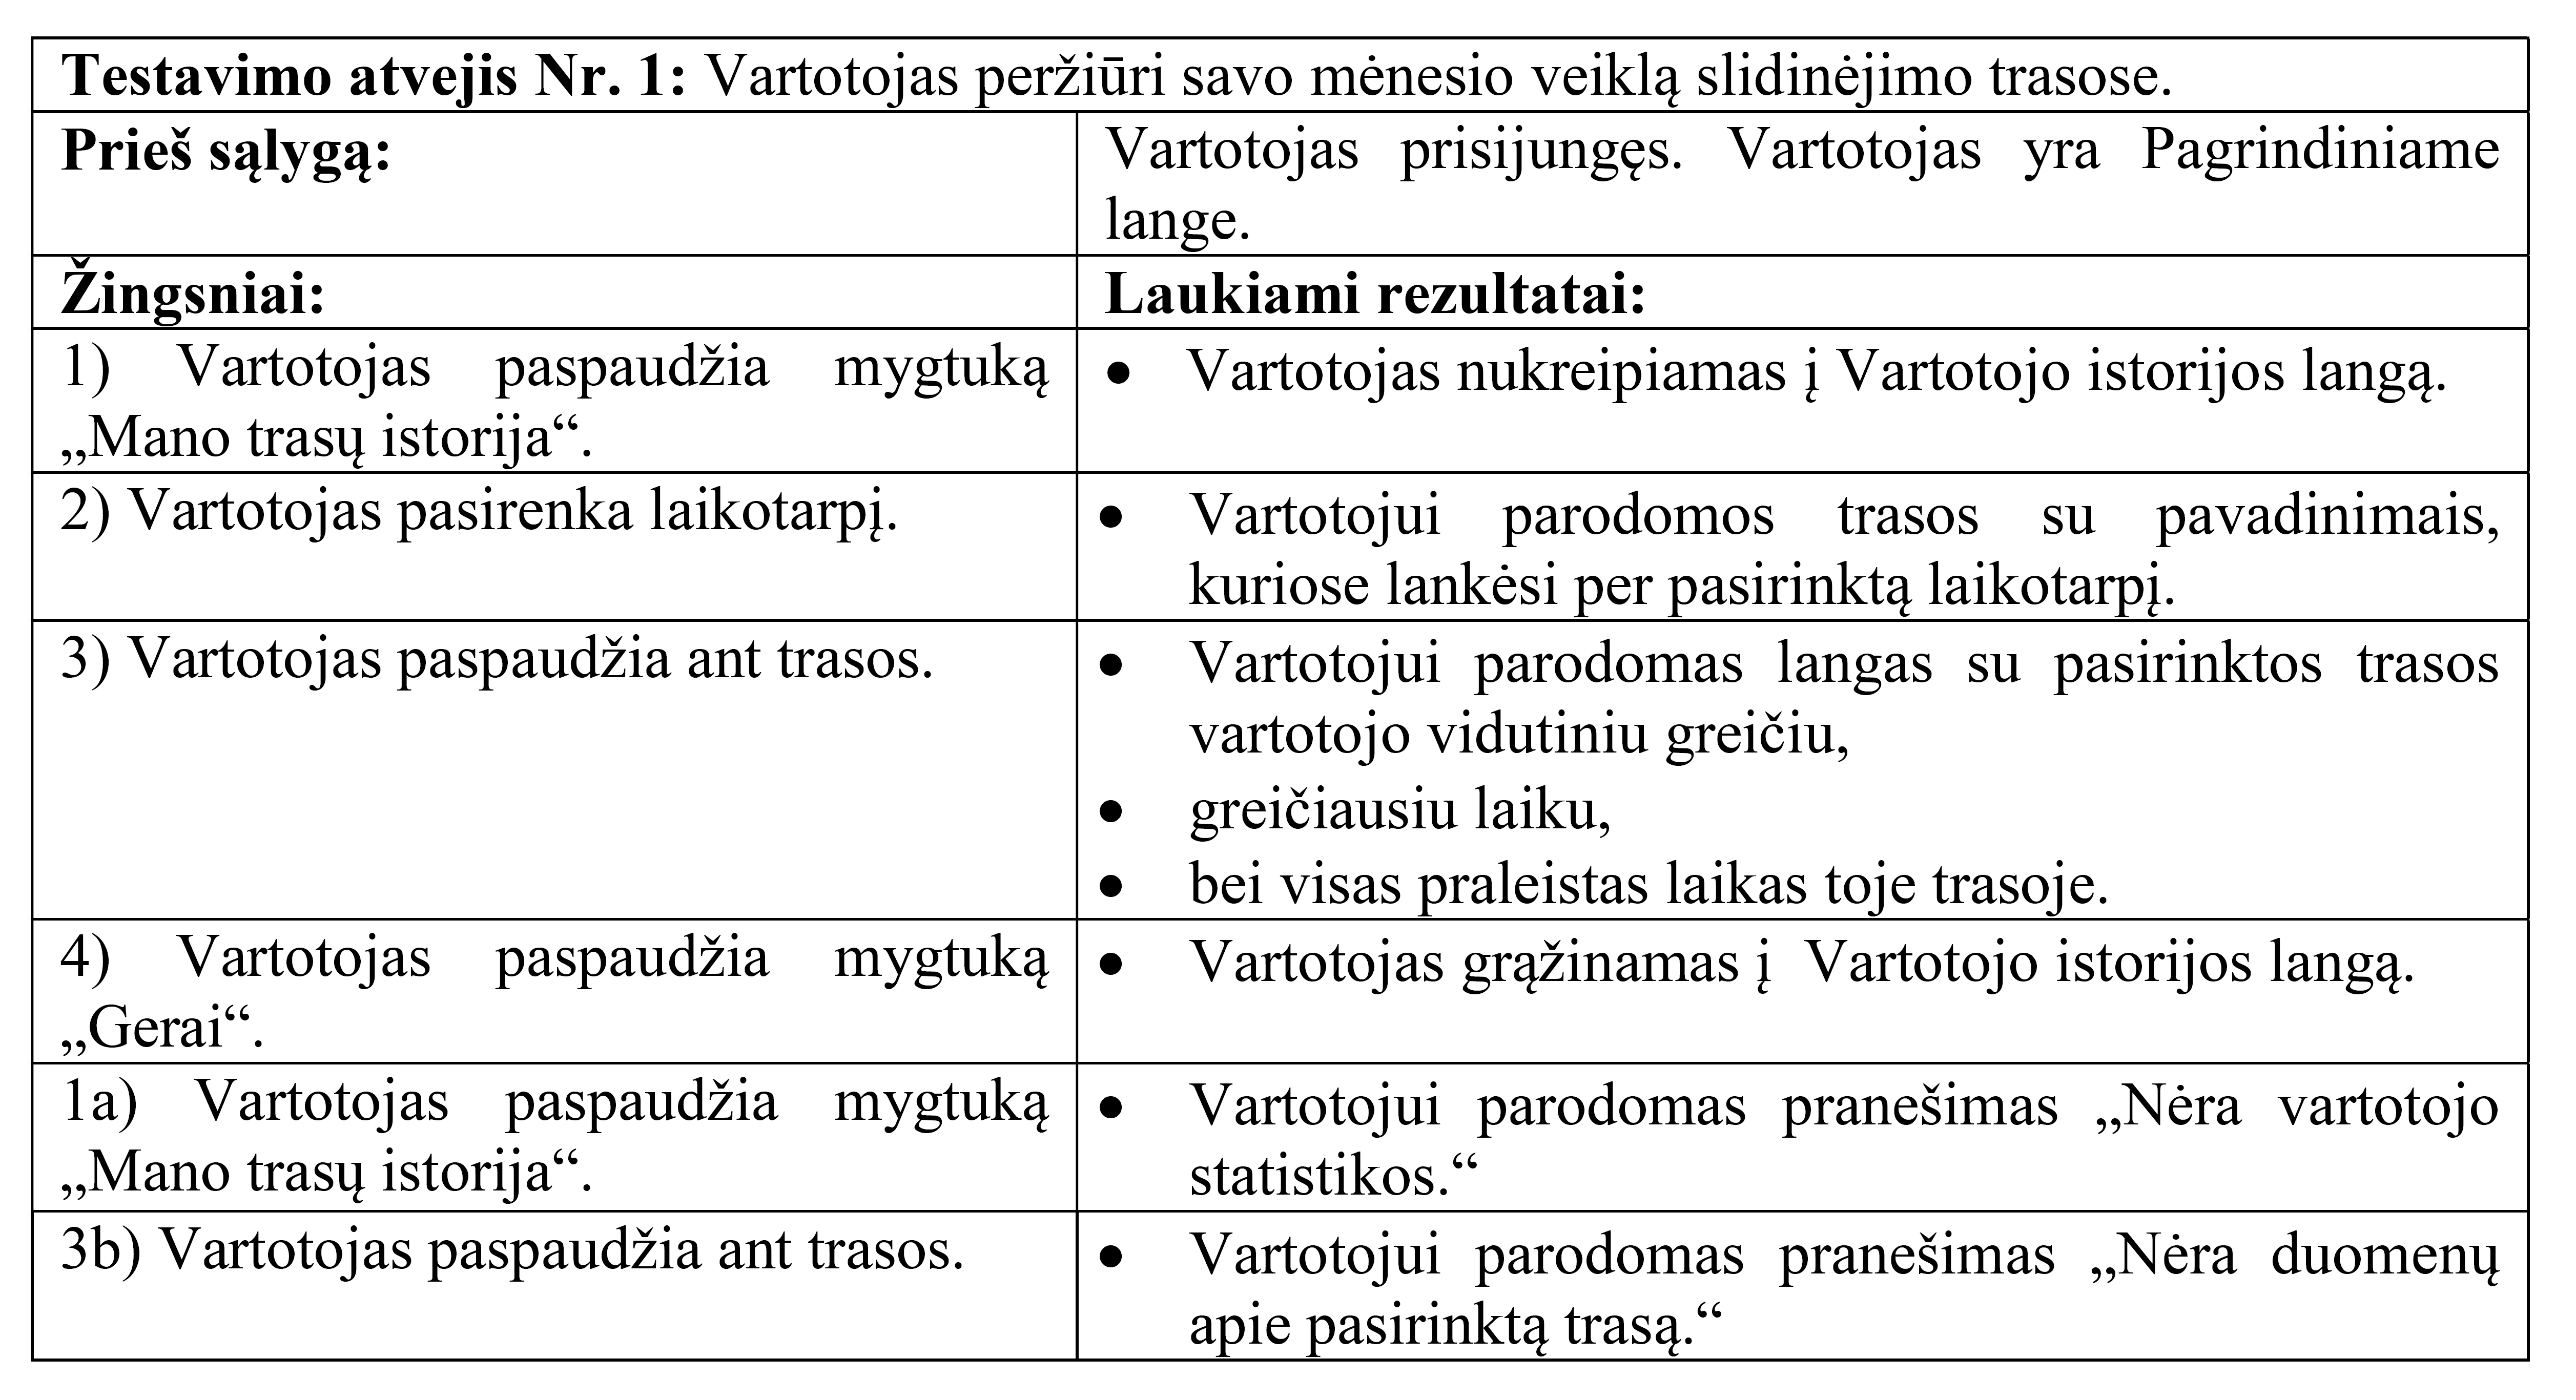
\includegraphics[width=1\textwidth]{test1.png}
    				\caption{Testas: Vartotojas peržiūri savo mėnesio veiklą}
    				\label{fig:Testas: Vartotojas peržiūri savo mėnesio veiklą}
			\end{figure}
			
			\begin{figure}[h]
    				\centering
    				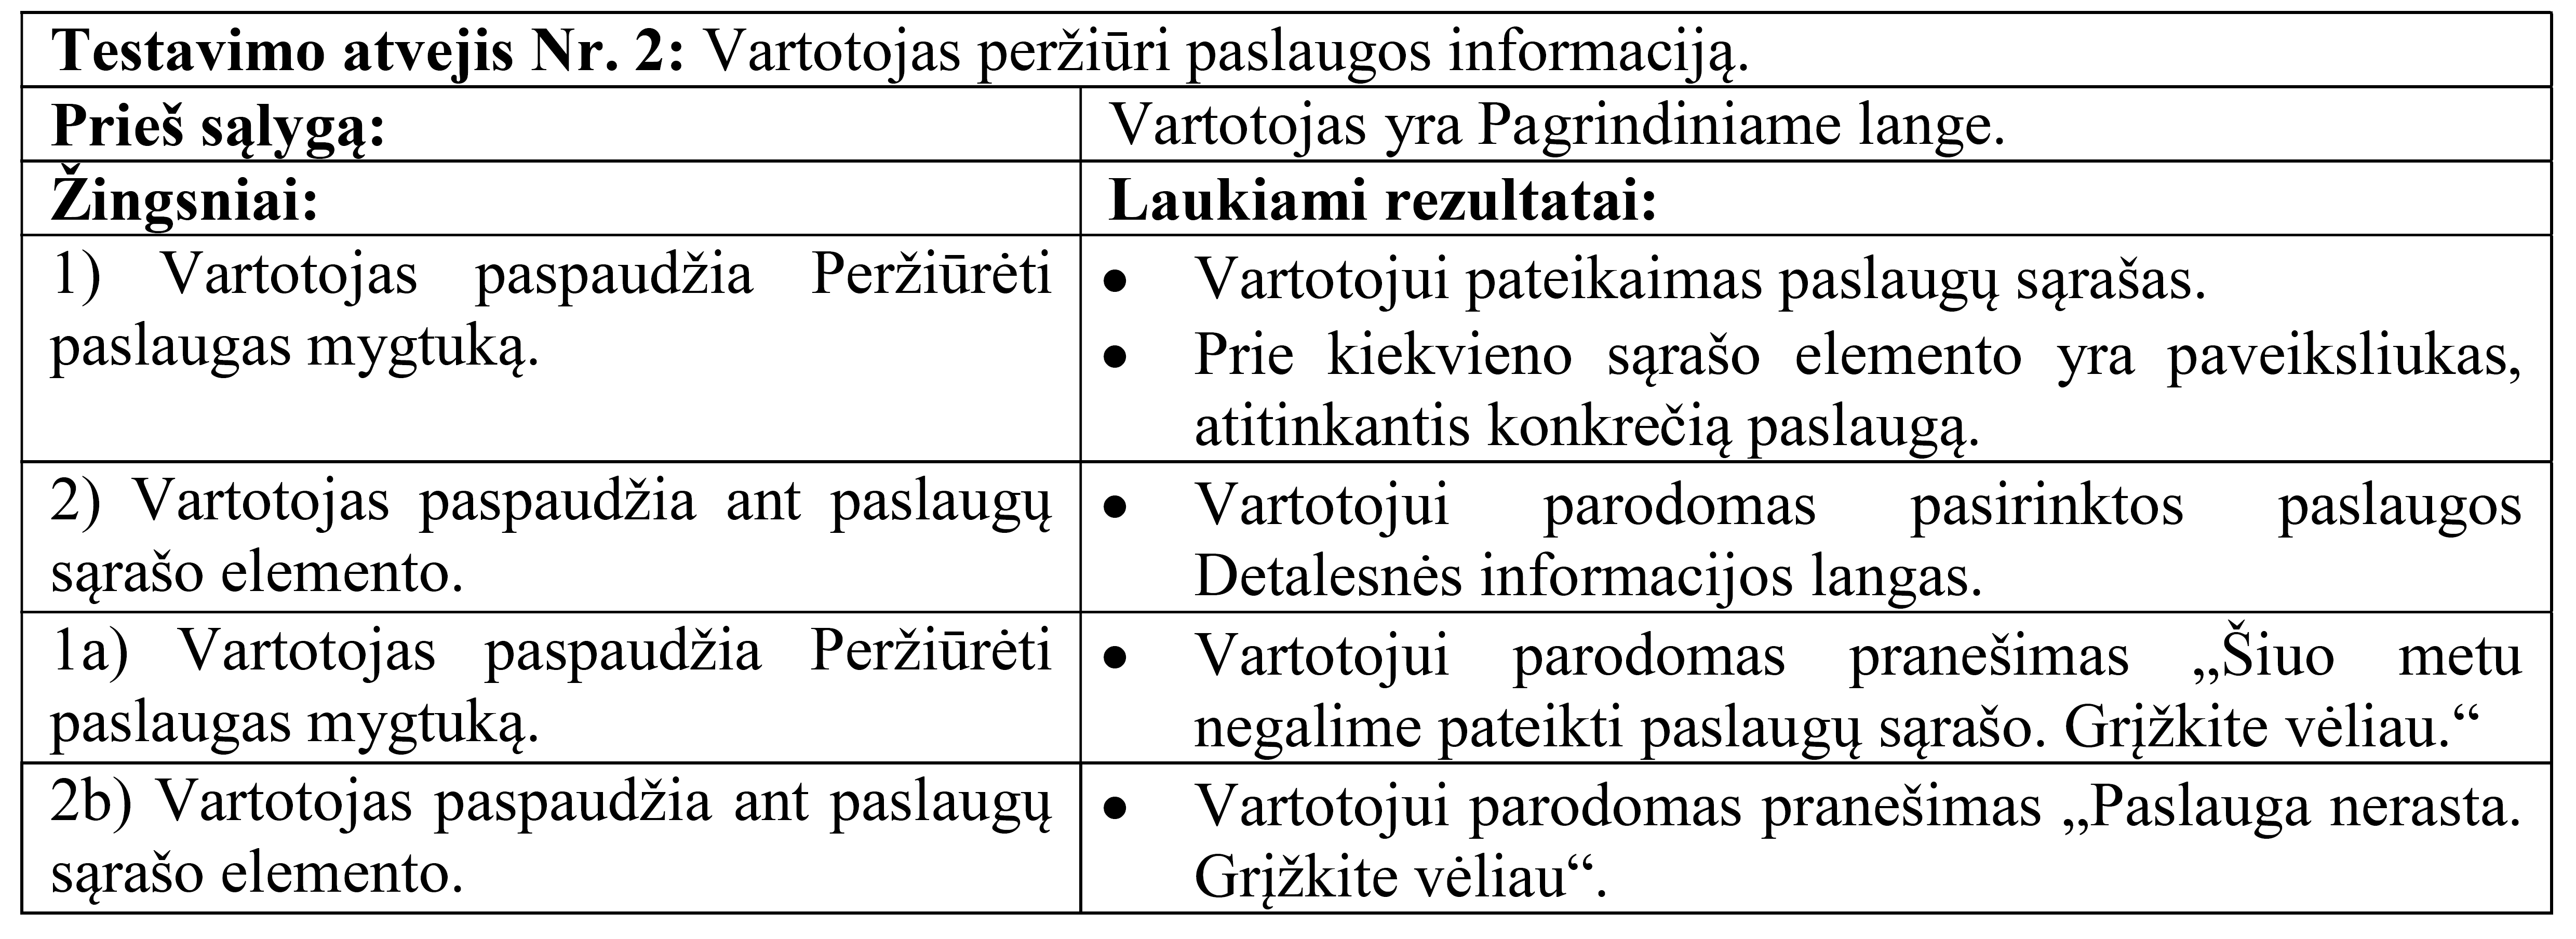
\includegraphics[width=1\textwidth]{test2.png}
    				\caption{Testas: Vartotojas peržiūri paslaugos informaciją}
    				\label{fig:Testas: Vartotojas peržiūri paslaugos informaciją}
			\end{figure}
			
			\begin{figure}[h]
    				\centering
    				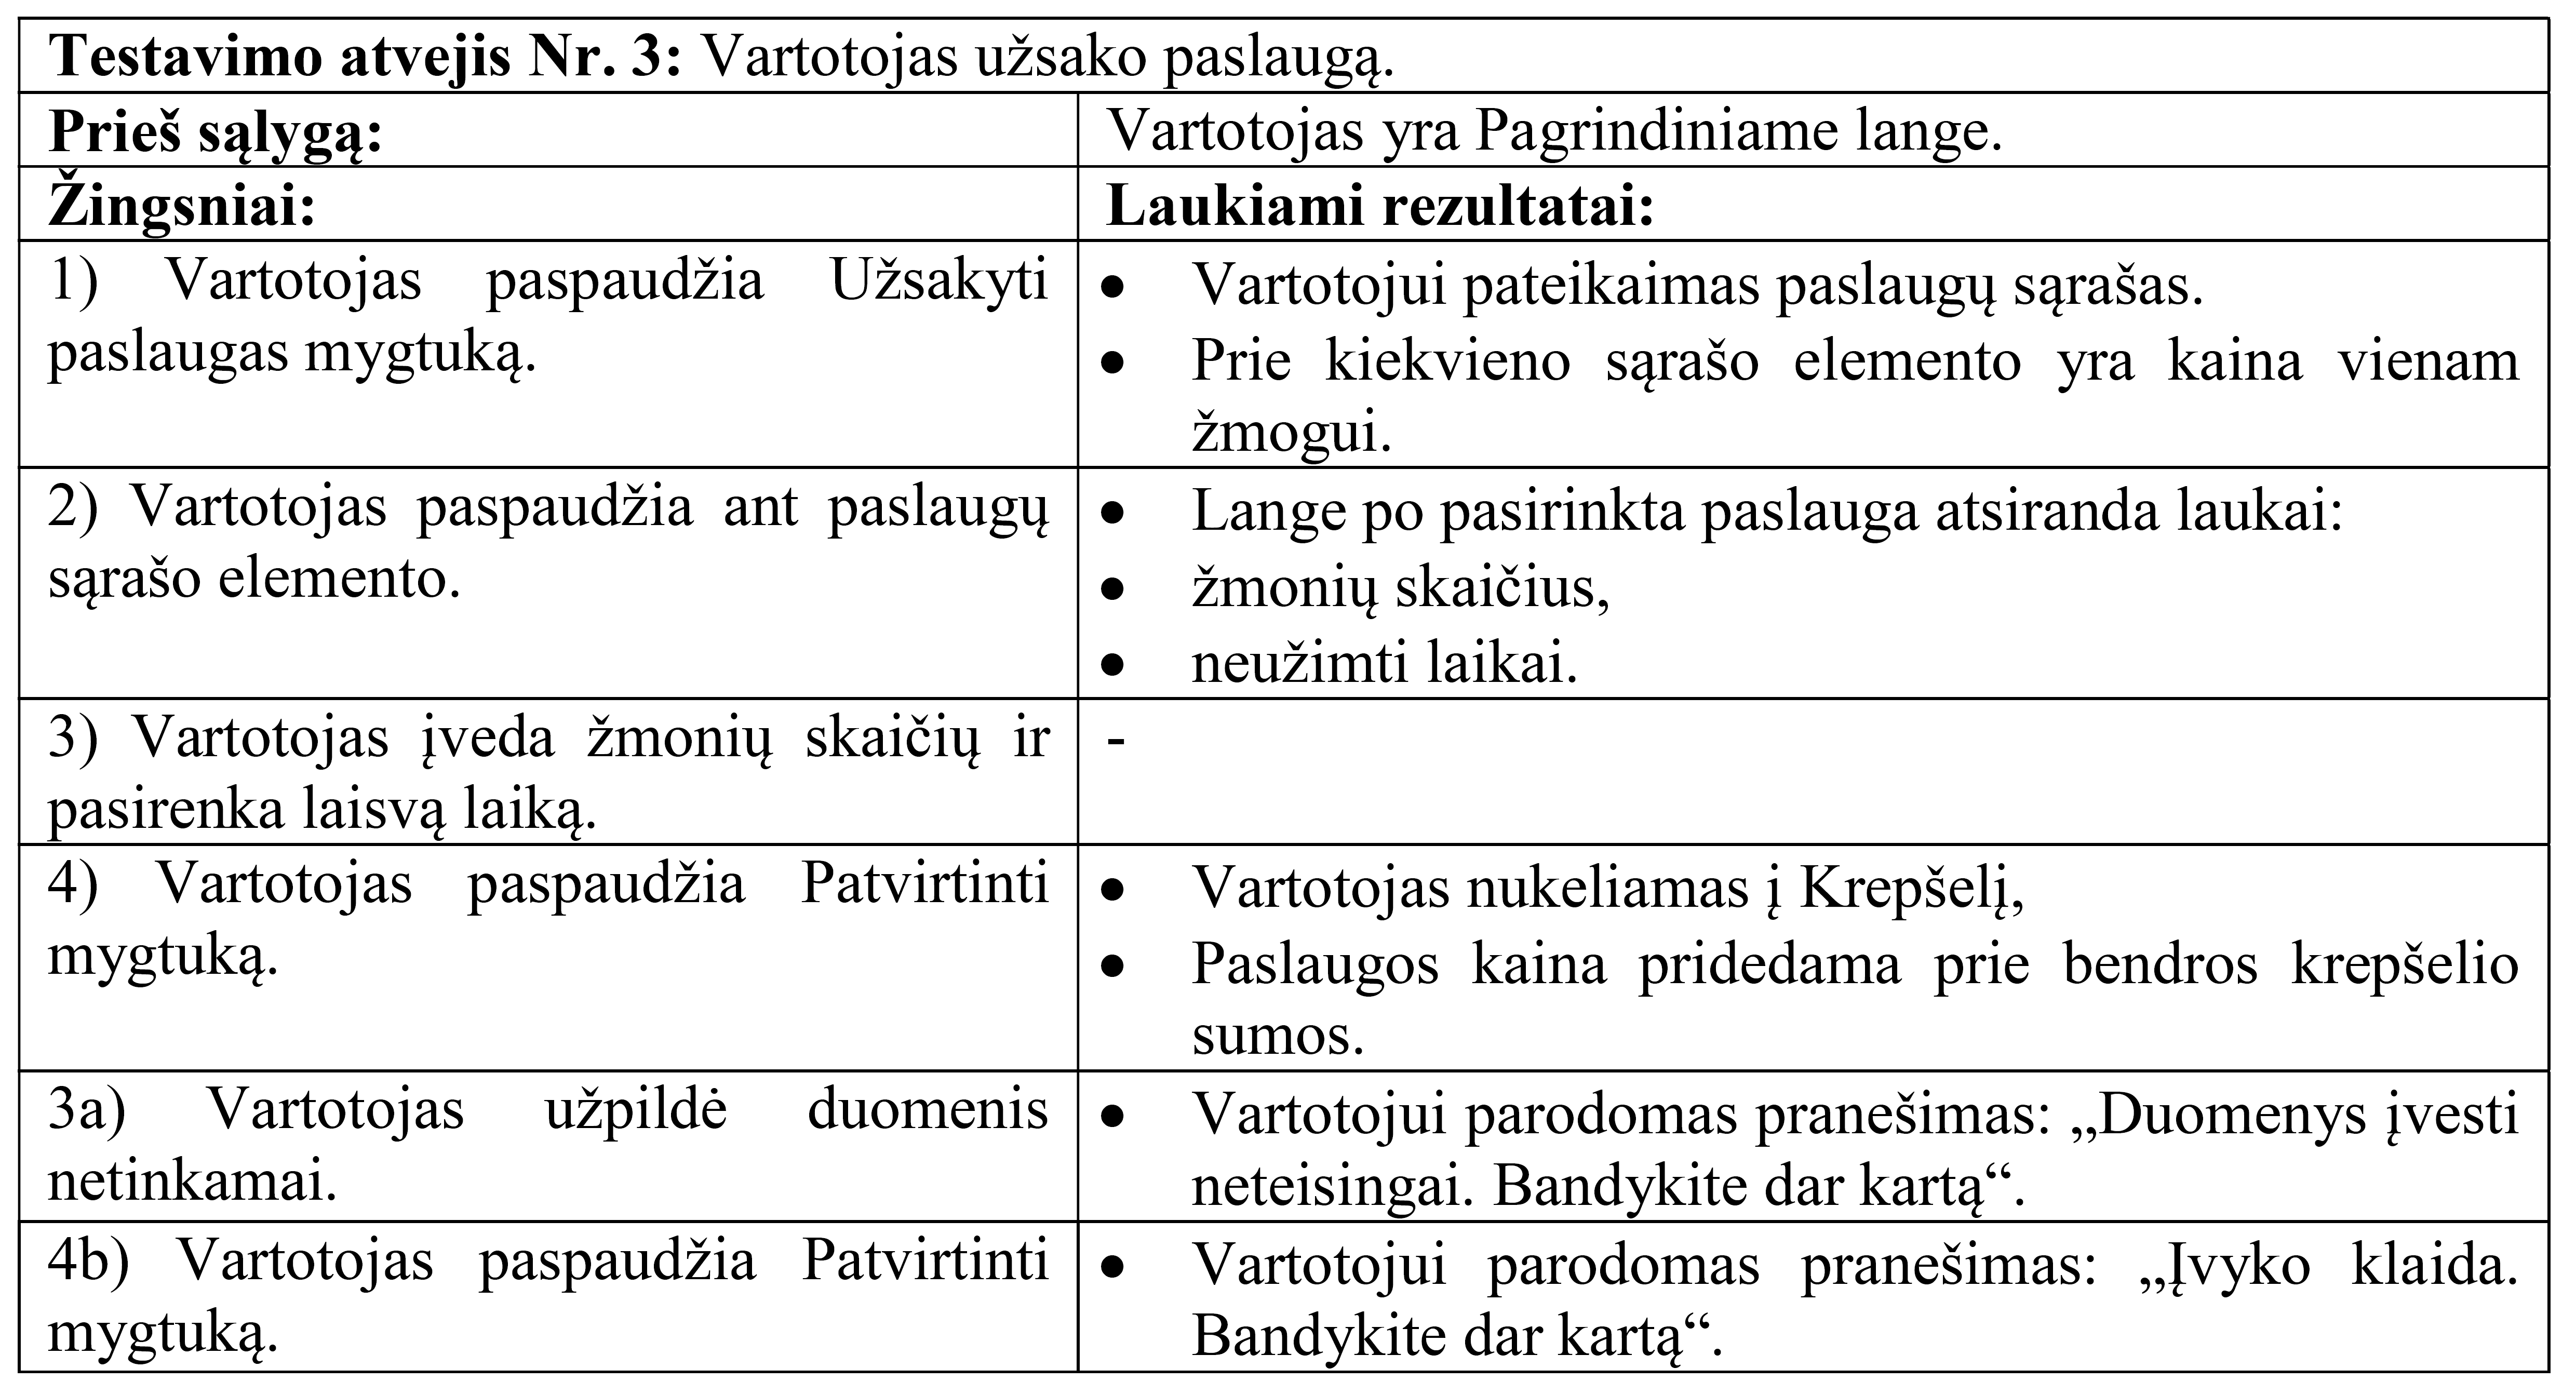
\includegraphics[width=1\textwidth]{test3.png}
    				\caption{Testas: Vartotojas užsako paslaugą}
    				\label{fig:Testas: Vartotojas užsako paslaugą}
			\end{figure}
			
			\begin{figure}[h]
    				\centering
    				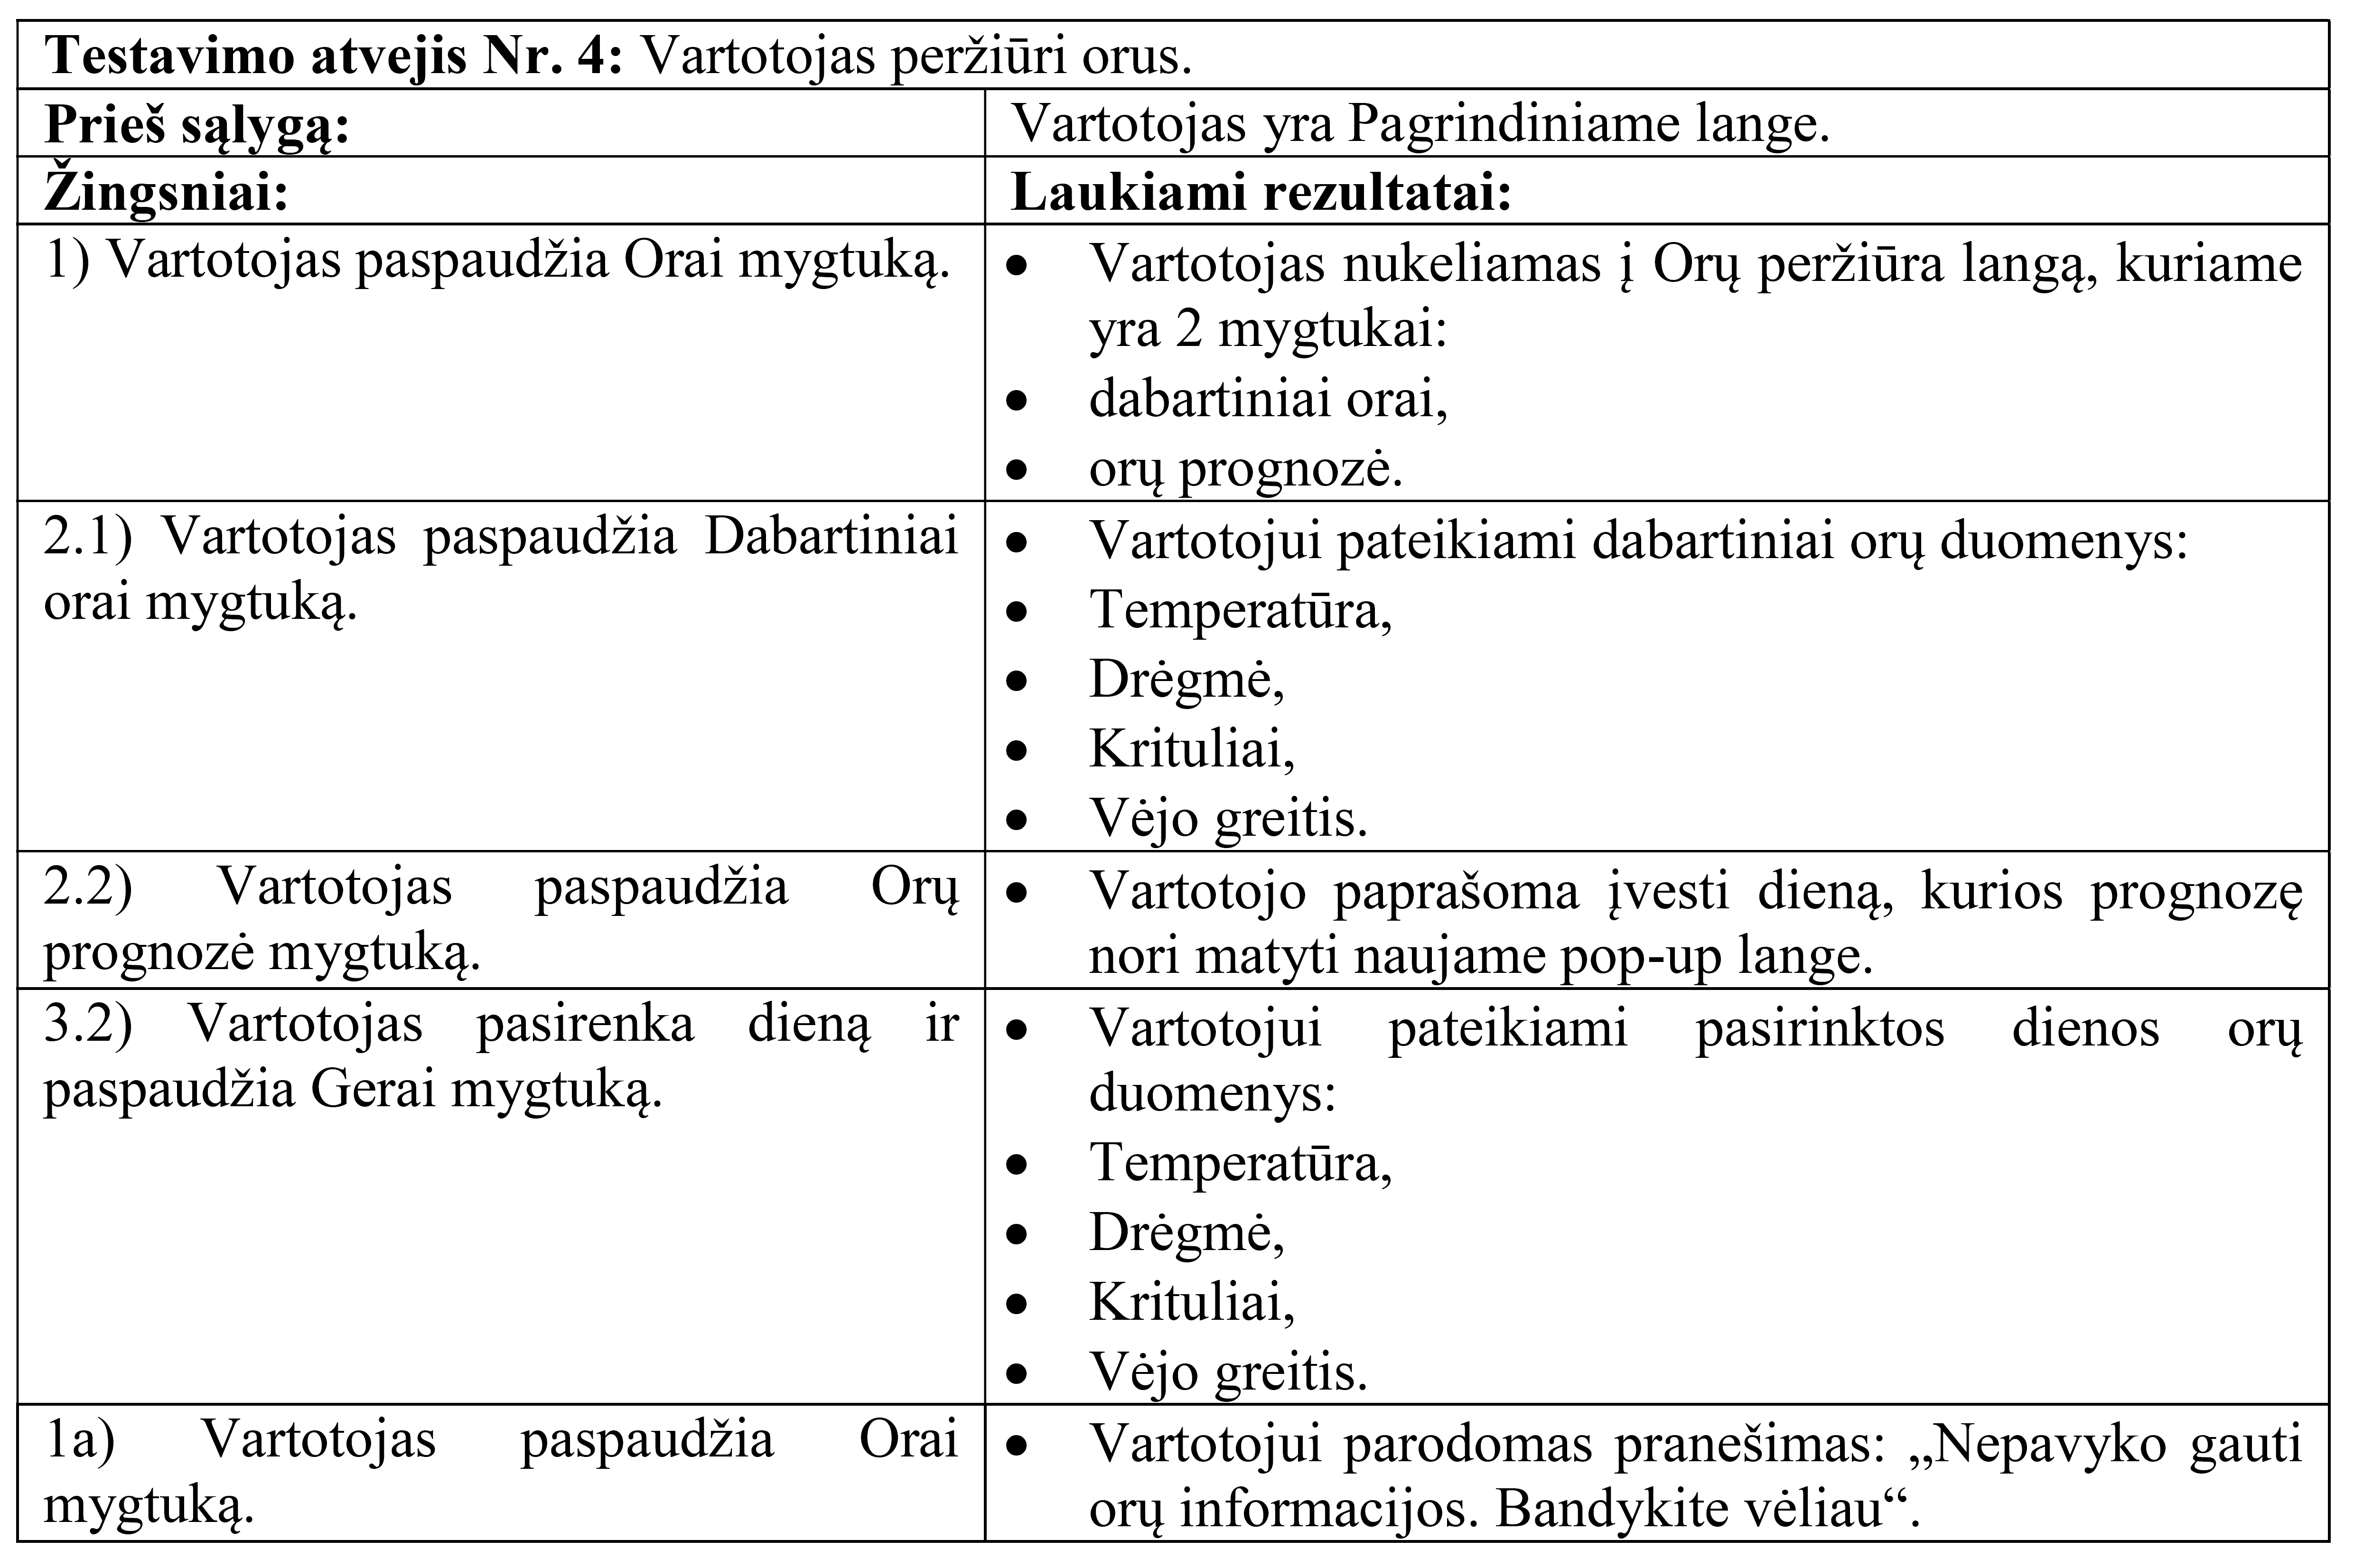
\includegraphics[width=1\textwidth]{test4.png}
    				\caption{Testas: Vartotojas peržiūri orus}
    				\label{fig:Testas: Vartotojas peržiūri orus}
			\end{figure}
			
			\begin{figure}[h]
    				\centering
    				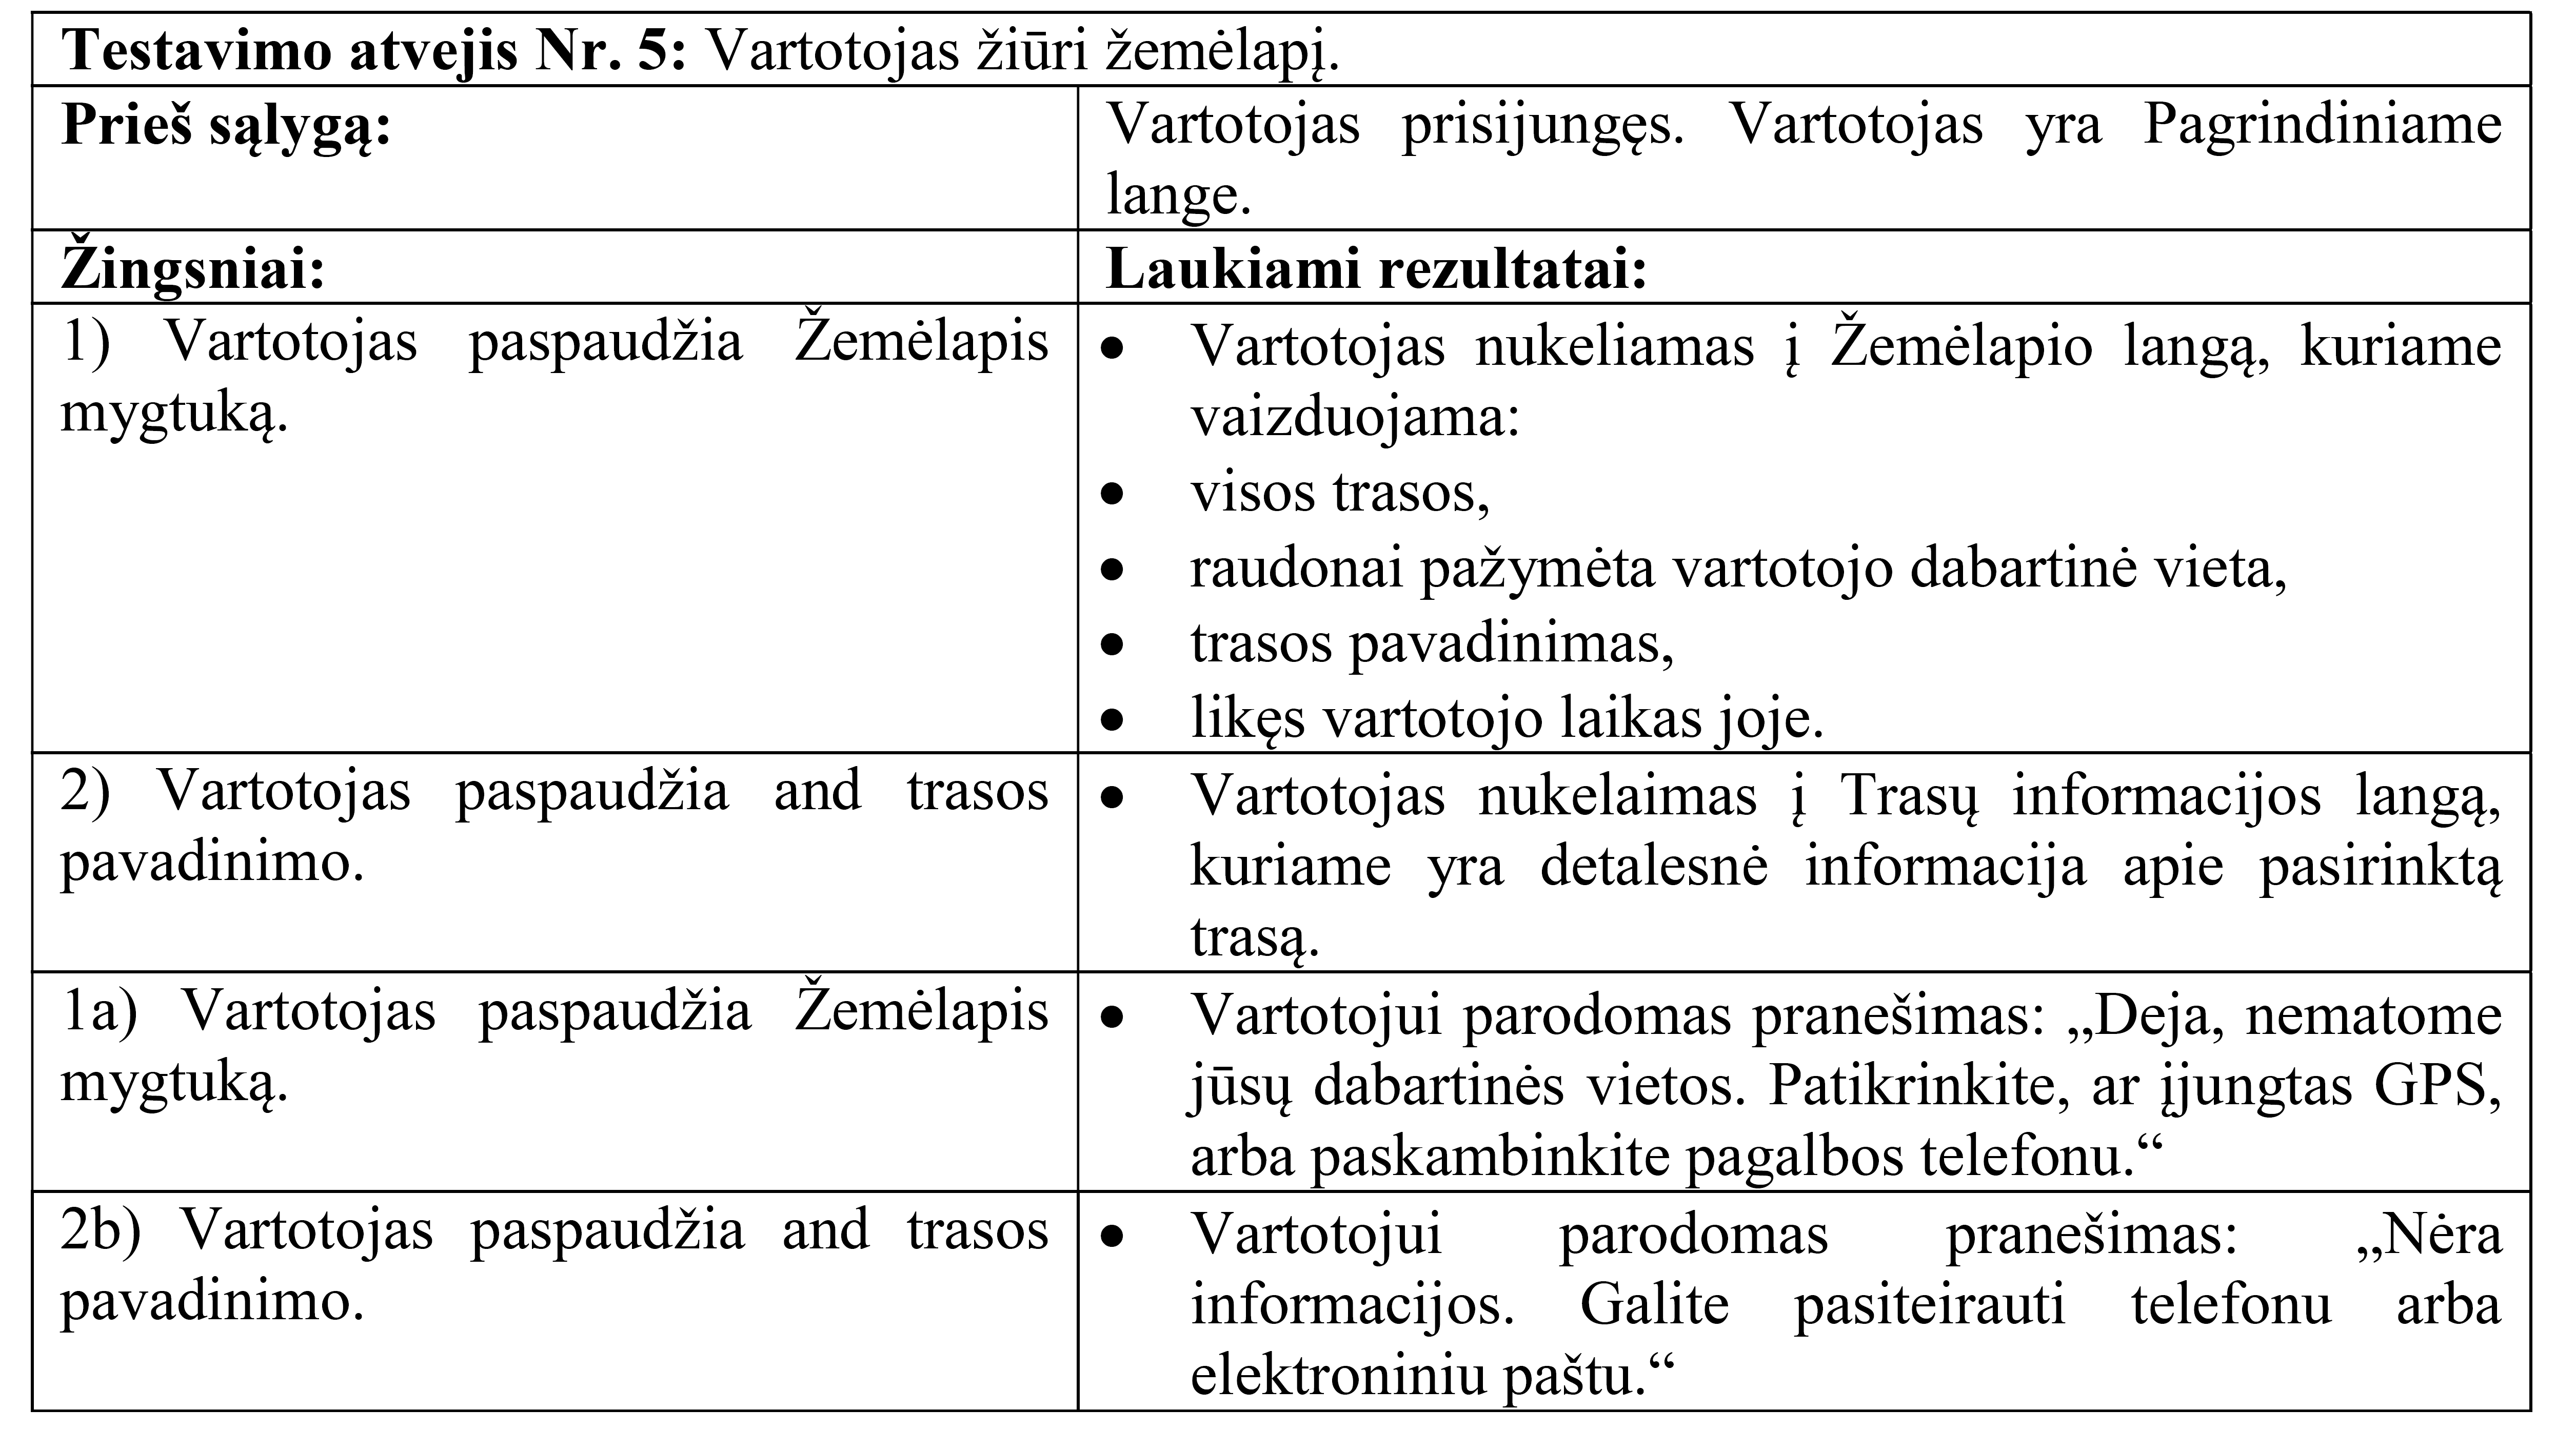
\includegraphics[width=1\textwidth]{test5.png}
    				\caption{Testas: Vartotojas žiūri žemėlapį}
    				\label{fig:Testas: Vartotojas žiūri žemėlapį}
			\end{figure}
			
			\begin{figure}[h]
    				\centering
    				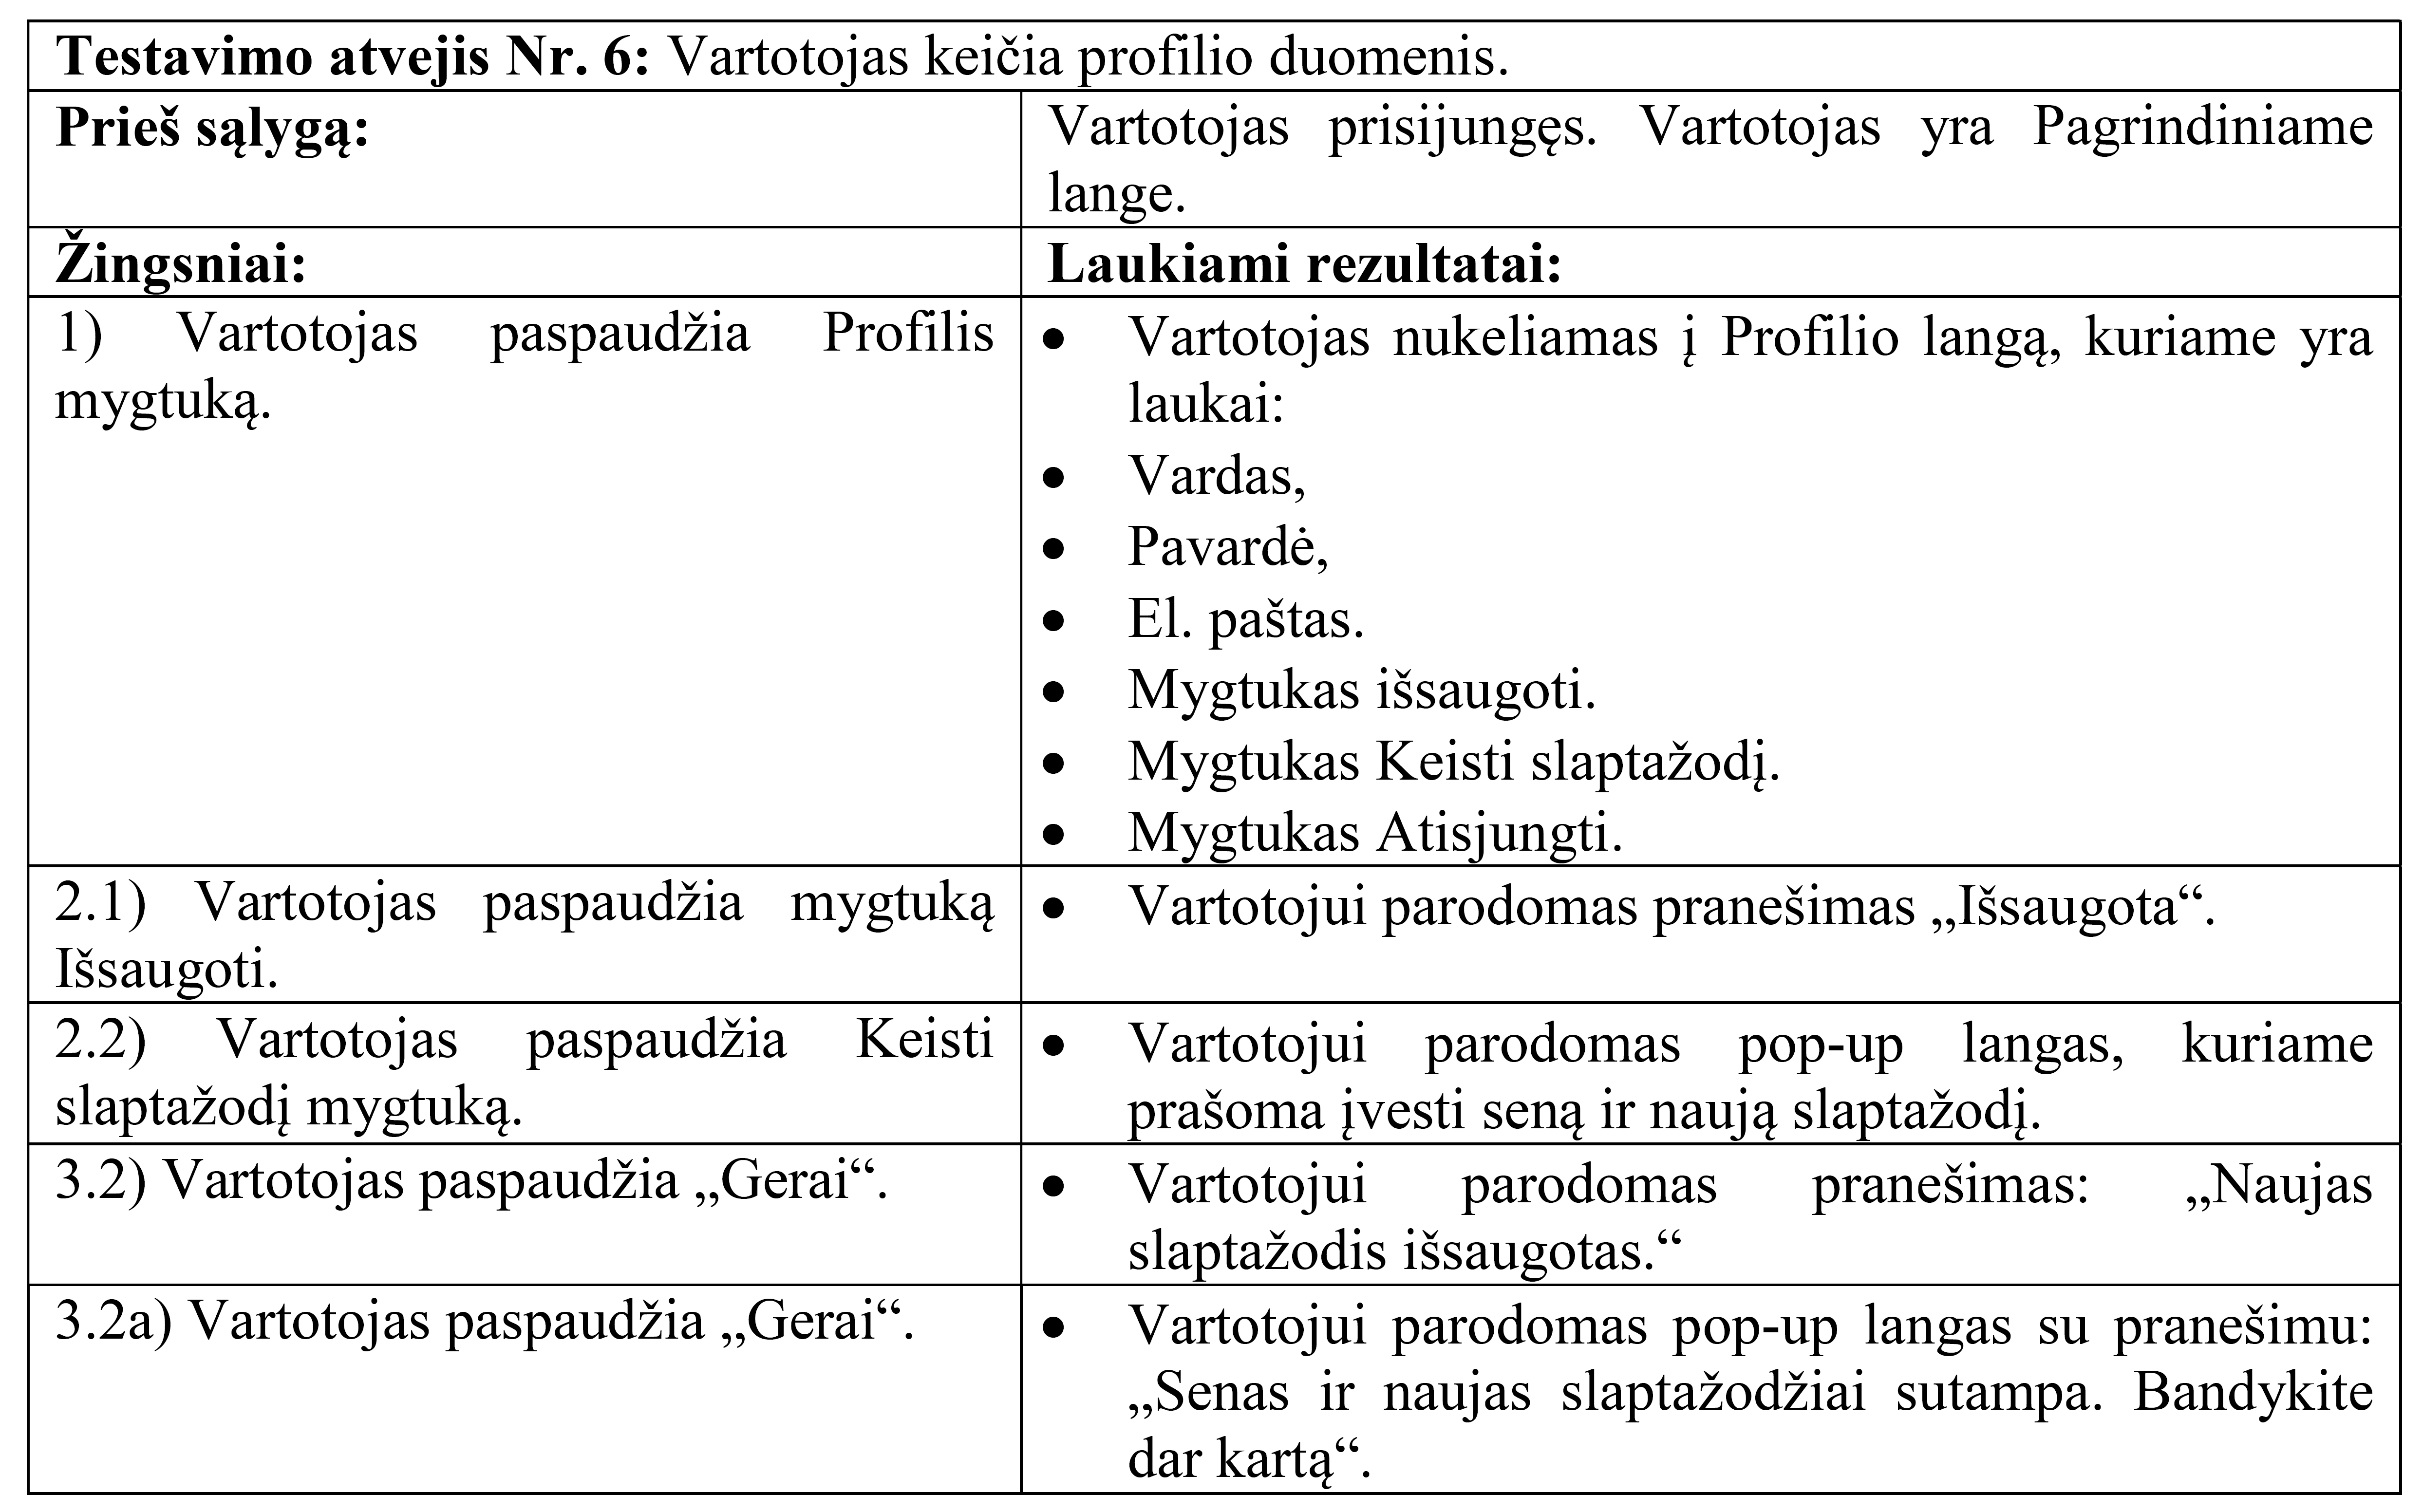
\includegraphics[width=1\textwidth]{test6.png}
    				\caption{Testas: Vartotojas keičia profilio duomenis}
    				\label{fig:Testas: Vartotojas keičia profilio duomenis}
			\end{figure}

\section{Sistemos techninė architektūra}
	\subsection{Sistemos komponentų diagrama}
			\begin{figure}[h]
    				\centering
    				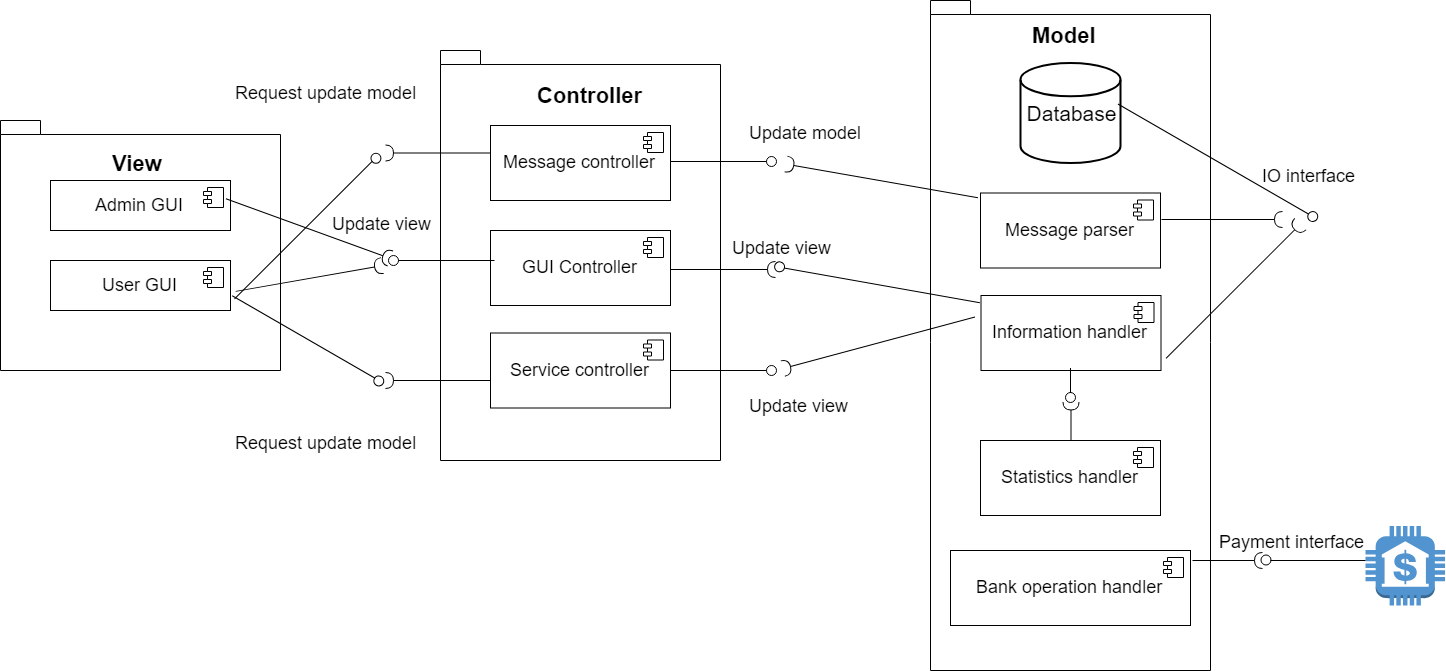
\includegraphics[width=1\textwidth]{KomponentuDiagrama.png}
    				\caption{Komponentų diagrama}
    				\label{fig:Komponentų diagrama}
			\end{figure}

	Sistema išskaidyta į 3 sluoksnius: View, Controller ir Model. View sluoksnyje talpiname vartotojo ir administratoriaus grafinius interfeisus, kurie bendrauja su Controller esančiais komponentais. Controller sluoksnyje esantys komponentai yra tarpiniai tarp grafinio interfeiso ir back-end. Komponentai, esantys jame, gavę grafinio interfeiso signalus juos apdoroja ir kreipiasi į Model, kuriame esantys komponentai pagrinde skirti duomenų bazės redagavimui. Norint atvaizduoti atnaujintą informaciją vartotojui, Model esantys komponentai perduoda informaciją į Controller ir pastarasis perduoda informaciją View, kur ją išvysta vartotojas.
	\subsection{Išdėstymo diagrama}
			\begin{figure}[h]
    				\centering
    				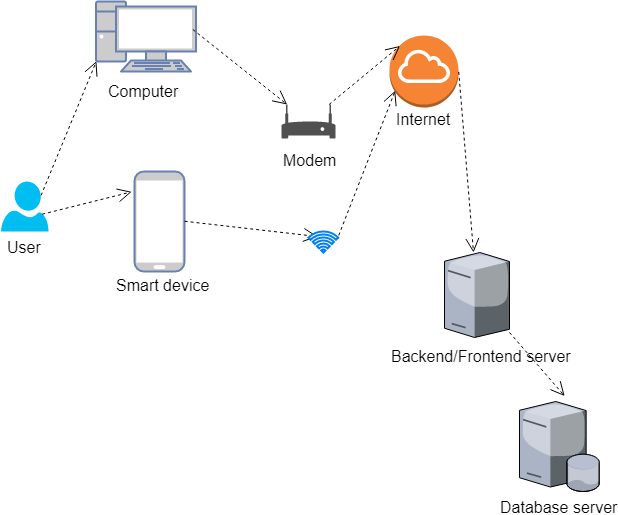
\includegraphics[width=0.75\textwidth]{Deployment.png}
    				\caption{Išdėstymo diagrama}
			\end{figure}

\section{Sistemos realizacija}
	\subsection{Duomenų bazės schema}
	\begin{figure}[h]
    				\centering
    				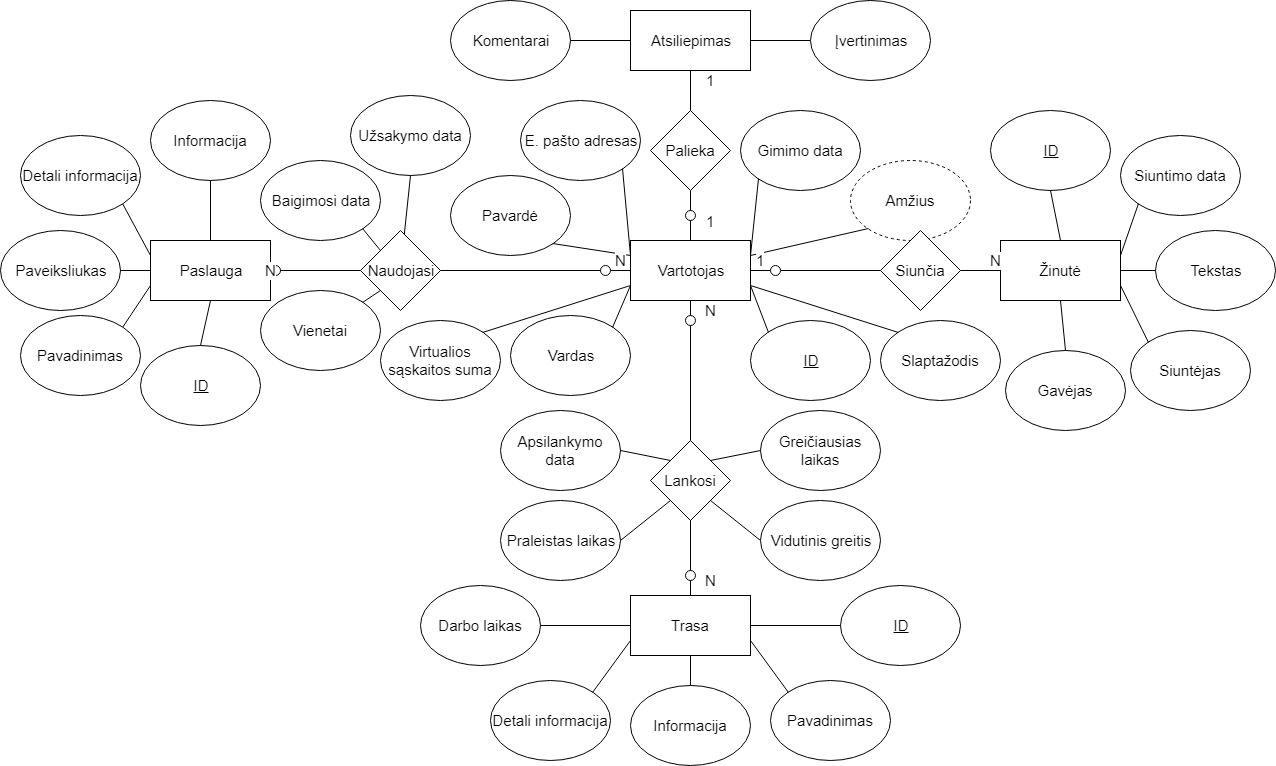
\includegraphics[width=1\textwidth]{Database2.png}
    				\caption{Duomenų bazės schema}
			\end{figure}
	\subsection{Pradiniai programų kodai ir aprašas}

\section{Reikalavimų specifikacija}

\section{Žodynas}
\begin{enumerate}
	\item Internetinė aplikacija - Mūsų kuriama android programėlė
	\item Administratorius - Sistemą prižiūrintis žmogus
	\item Vartotojas - Slidinėjimo kurorto klientas, naudojantis programėlę
	\item Susirašinėjimas - Dviejų vartotojų žinučių grandinė
	\item Virtuali piniginė - Piniginė, kurioje esančiais pinigais galima atsiskaityti už pramogas
	\item Sekimo prietaisas - Įrenginys, siunčiantis savo poziciją sistemai
	\item Atsiskaitymų sistema - Sistema, kuri apdoroja bankinius pinigų pervedimus
	\item Duomenų bazė - Organizuota duomenų struktūra
	\item Vartotojo statistika - Duomenys, renkami apie vartotoją
	\item Sutartys - Rašytinis susitarimas tarp vartotojo ir slidinėjimo kurorto
	\item Kurorto statistika - Duomenys renkami apie kurortą
	\item DAO - Data Access Object
\end{enumerate}

\end{document}